%% -*- coding: utf-8; -*-

% Use 'digital' option to enable back references. This option is recommended for digital pdf version
%\documentclass[phd,american,digital]{thesispuc}%english thesis
%\documentclass[mscr,american]{thesispuc}%english dissertation
%\documentclass[phd,brazilian]{thesispuc}%tese em portugês
\documentclass[msc,brazilian]{thesispuc}%disseretação em portuguŝ


%%%
%%% Additional Packages
%%%
\usepackage{tabularx}
\usepackage{multirow}
\usepackage{multicol}
\usepackage{colortbl}
\usepackage[%
    dvipsnames,
    svgnames,
    x11names,
    fixpdftex,
    table
]{xcolor}
\usepackage{numprint}
\usepackage{textcomp}
\usepackage{booktabs}
\usepackage{amsmath}
\usepackage{enumitem}
\usepackage{amssymb}
% ABNT reference style package. The current style is the alphabetical order, if you need
% change to citation order, change in the line above 'alf' to 'num', also at the end replace
% bibliographystyle with the commented version.
\usepackage[num]{abntex2cite}
%\usepackage{tikz}
%\usepackage[linesnumbered, ruled, vlined]{algorithm2e}
%\usepackage{pgfplots,pgfplotstable} 
%\usepackage{array}

% ADICIONADAS POR DANIEL
\usepackage{multirow}
\usepackage{longtable}
\usepackage{mathtools}

%% numprint 
\npthousandsep{.}
\npdecimalsign{,}

%% ThesisPUC option
%\tablesmode{fig} %% [nada, fig, tab ou figtab]
%\algoritmsmode{none} %% [none ou use] %% Default is [use]
%\codesmode{none} %% [none ou use] %% Default is [use]
%\abreviationsmode{none} %% [none ou use] %% Default is [use]

\tablesmode{figtab}

\algorithmsmode{none}
\codesmode{use}
\abreviationsmode{none}

% \makeatletter  \renewcommand\@biblabel[1]{#1}  \makeatother

%%%
%%% Counters
%%%

%% uncomment and change for other depth values
\setcounter{tocdepth}{1}
%\setcounter{lofdepth}{3}
%\setcounter{lotdepth}{3}
%\setcounter{secnumdepth}{3}

%%%
%%% Misc.
%%%

\usecolour{true}
%% \graphicspath{ {./figuras/} }
%% https://www.overleaf.com/learn/latex/Inserting_Images
\citebrackets[]

\renewcommand{\arraystretch}{1.5}


%%%
%%% Titulos
%%%

\autor{Daniel Schreiber Guimarães}
\autorR{Guimarães, Daniel Schreiber}

\advisor{Marcos Vianna Villas}{Prof.}
\advisorR{Villas, Marcos Vianna}
% If the advisor's department is different from author's department, uncomment the next line and type the correct name and acronym of advisor's institution.
%\advisorInst{institution name}{acronym}

%\coadvisor{Otávio da Fonseca Martins Gomes}{Dr.}
%\coadvisorR{da Fonseca Martins Gomes, Otávio}
%\coadvisorInst{Centro de Tecnologia Mineral}{CETEM/MCTI}

\title{Sistema de recomendação de disciplinas para matrícula de um aluno da PUC-Rio}
\titleuk{Course recommendation system for the enrolling of a PUC-Rio student}

%%\subtitulo{Aqui vai o subtitulo caso precise}

\day{24}
\month{Novembro}
\year{2023}

\city{Rio de Janeiro}
\CDD{004} 
\department{Informática}
\program{\mbox{Engenharia} da \mbox{Computação}}
\school{\mbox{Engenharia} da \mbox{Computação}}
\university{Pontifícia Universidade Católica do Rio de Janeiro}
\uni{PUC-Rio}


%%%
%%% Jury
%%%

\jury{%
  \jurymember{Sérgio Lifschitz}{Prof.}
    {Departamento de Informática}{PUC-Rio}
  \jurymember{Augusto Baffa}{Prof.}
    {Departamento de Informática}{PUC-Rio}
}


%%%
%%% Personal Resume
%%%

\resume{%
% If it fit in one line use this command:
\makebox[\textwidth][s]{Graduando em Engenharia da Computação na PUC - Rio}%
% If not just type your resume without any special command 
}

%%%
%%% Acknowledgment (REMINDER TO SCHOLARSHIP STUDENTS. Do not forget to thank the agencies that supported your work.)
%%% REMOVIDO POR DANIEL
%%%
% \acknowledgment{%
% \noindent To my adviser Professor Marcelo Gattass for the stimulus and partnership
% to carry out this work.
% \bigskip

% \noindent To CNPq and PUC-Rio, for the aids granted, without which this work does not
% could have been accomplished.
% \bigskip
% }


%%%
%%% Catalog prekeywords
%%%

\catalogprekeywords{%
  \catalogprekey{Informática}%
}

%%%
%%% Keywords - Don't use % at the end of /key dfinition
%%%

\keywords{%
  \key{Recomendação}
  \key{Disciplinas}
  \key{Algoritmo}
}

\keywordsuk{%
  \key{Recommendation}
  \key{Courses}
  \key{Algorithm}
}


%%%
%%% Abstract
%%%

\abstract{%
A PUC-Rio permite que os alunos escolham quais disciplinas irão cursar no próximo semestre, mas a tomada de decisão não é uma tarefa fácil, visto que as informações
relevantes como dificuldade da matéria, horários disponíveis ou professores disponíveis não são triviais de se encontrar. Esse projeto de graduação é referente
a um sistema que oferece uma plataforma para alunos montarem suas grades, avaliarem disciplinas e professores, e receberem recomendações de disciplinas para serem
cursadas.
} 

\abstractuk{%
PUC-Rio allows students to choose which courses they may take in the next semester, but decision-making is not an easy task, given that relevant informação such 
as the difficulty of the subject, available schedules, or available professor is not trivial to find. This graduation project is related to a system that provides
a plataform for students to build their schedules, evaluate courses and professors, and receive recommendations for courses to be taken.
}


%%%
%%% Dedication
%%%

\dedication{%
  Para os meus pais, que\\nunca deixaram de me ajudar.
}

%%%
%%% Epigraph (removido manualmente pelo thesispuc.cls)
%%%

% \epigraph{%
% }
% \epigraphauthor{Wassily Kandinsky}
% \epigraphbook{Regards sur le passé}


\begin{document}
  % -*- coding: utf-8; -*-

\chapter{Introdução}

A cada semestre, um aluno que está fazendo graduação no Departamento de Informática da PUC-Rio precisa fazer a sua matrícula em disciplinas oferecidas pela universidade para os próximos seis meses. Apesar de algumas restrições como pré-requisitos de disciplinas, o aluno tem ampla liberdade de escolher as disciplinas que melhor se encaixam na sua grade horária. Essa liberdade é uma vantagem devido à disponibilização de uma grade horária flexível para o aluno, porém precisa de um maior esforço de pesquisa e organização deste aluno para que a sua matrícula no próximo período seja feita de forma eficaz segundo critérios do próprio aluno. 

A motivação desse projeto é o estudo, planejamento e desenvolvimento de um sistema de recomendação de disciplinas para o próximo período que auxilie o aluno em sua matrícula ao sugerir interativamente disciplinas com base em dados fornecidos pela universidade e por avaliações informadas por alunos.
  % -*- coding: utf-8; -*-

\chapter{Situa{\c c}\~ao Atual}
\label{cha:Situa{\c c}\~ao Atual}

\section{Serviços disponibilizados}

O microhorario\footnote{https://www.puc-rio.br/microhorario} é um serviço disponibilizado pela universidade para consultar informações das disciplinas do semestre atual. Este possui uma interface simples que pode ser visualizada na figura \ref{fig:microhorario}. Essa interface permite filtrar disciplinas por seus atributos como nome, código, professor e departamento. Porém, essa interface não é personalizada com relação ao aluno, ou seja, não exibe as disciplinas que o aluno em específico ainda não cursou ou que o aluno não pode cursar devido à pré-requisitos.

\begin{figure}[h]
    \begin{center}
    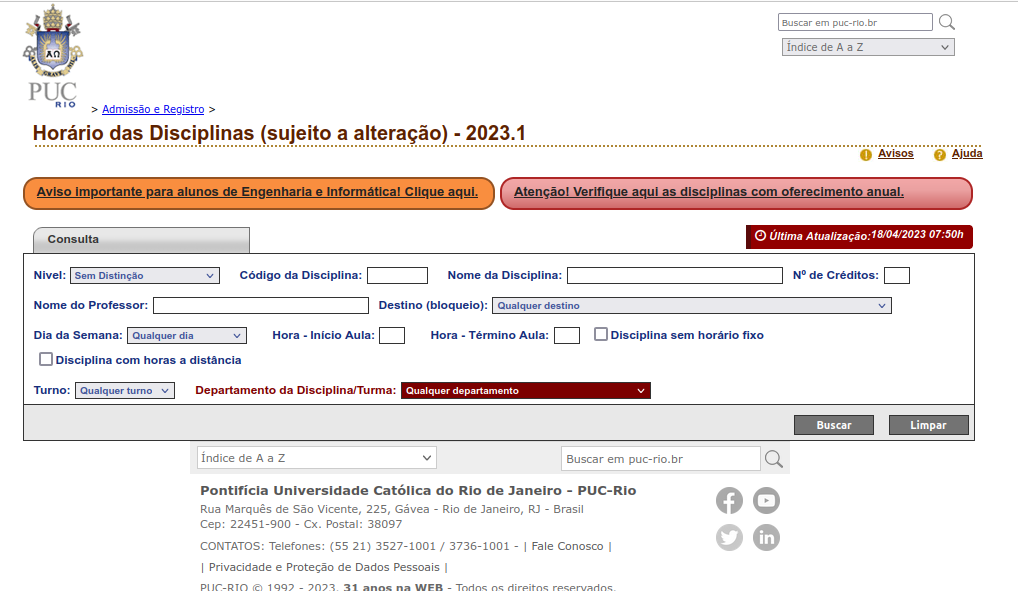
\includegraphics[width=300pt]{figuras/microhorario}
    \caption{Interface do \textit{microhorario}}
    \label{fig:microhorario}
    \end{center}
\end{figure}

Para consultar a grade recomendada e os pré-requisitos, o aluno de engenharia de computação precisa acessar um documento\footnote{http://www.inf.puc-rio.br/wordpress/wp-content/uploads/2023/01/\\Grade\_Eng\_comp\_2023.pdf} presente na página do departamento ou acessar o currículo disponibilizado na página da universidade. Outros cursos disponibilização documentos semelhantes em páginas diferentes. A grade recomendada possui os nomes das disciplinas e seus pré-requisitos, mas não contém a disponibilidade do próximo período.

Além disso, as disciplinas eletivas que o departamento oferece durante o semestre são anunciadas em diferentes veículos de comunicação, como e-mail, página da coordenação do curso, ou folhetos em corredores do departamento. Não há uma distribuição centralizada das ofertas de disciplinas eletivas, portanto o aluno pode não saber aonde procurar essas ofertas, e perder boas oportunidades por desconhecer o anúncio da disciplina eletiva.

No final de cada período, a universidade oferece um serviço de avaliação de disciplinas e professores, permitindo avalia-los em várias categorias. Porém, os resultados das avaliações não são disponíveis publicamente.

\section{Processo de matrícula}

A matrícula na PUC-Rio é um processo que dura vários dias. A universidade divulga o agendamento de matrícula, em que cada aluno recebe uma data e hora para realizar sua matrícula através do portal online do aluno. As datas possíveis abrangem um período de cinco dias. Durante o período de matrícula, o microhorario atualiza periodicamente para indicar quais turmas ainda possuem vagas disponíveis, e se houve o cadastro ou cancelamento de alguma outra disciplina durante este período.

Portanto, é comum que um aluno crie formas de planejamento próprias para conseguir organizar todo o fluxo de dependências, anotar as disciplinas que estão sendo oferecidas, assim como suas turmas e professores. Esses dados precisam estar em constante atualização durante o período de matrícula, conforme as vagas vão sendo preenchidas e a disponibilização de novas turmas ou disciplinas são anunciadas. Este é um processo que maximiza a qualidade da sua grade horária, mas demanda muito esforço e tempo. 

\begin{figure}[h]
  \begin{center}
  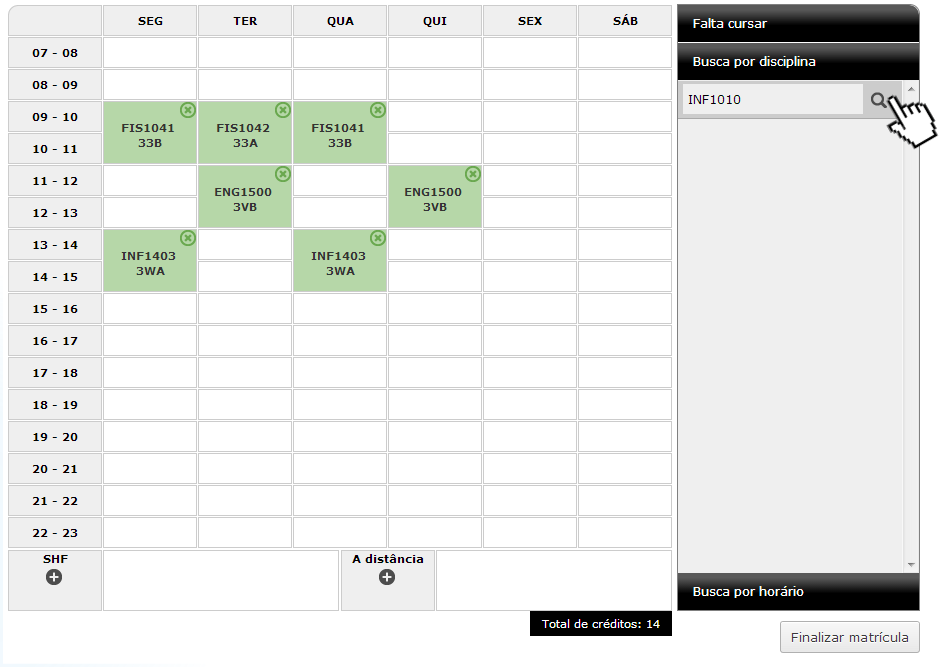
\includegraphics[width=250pt]{figuras/simulador}
  \caption{Interface do simulador}
  \label{fig:simulador}
  \end{center}
\end{figure}

A universidade disponibiliza por dois ou três dias um simulador de matrícula  antes do processo de matrícula em si. A interface do simulador é a mesma da matrícula, como pode ser observado na figura \ref{fig:simulador}, 
afim de o aluno poder simular a criação da sua grade de disciplinas para o próximo semestre. O simulador apresenta os dados das disciplinas atualizados conforme o microhorario, e os disponibiliza de três formas diferentes: buscas por disciplinas que faltam cursar no currículo do aluno, buscar por nomes de disciplinas e buscar por horários das turmas das 
disciplinas.\cite{doc-matricula}



\section{Estudos relacionados}

A escolha de disciplinas é um problema comum em universidades que possuem algum grau de flexibilidade na grade horária. Ng \& Linn\cite{crs-recs} desenvolveram um sistema de recomendação de disciplinas para a sua universidade chamado CrsRecs que utiliza análise de sentimento, pontuações de professores e disciplinas, e preferências que o aluno escolhe fornecer. A vantagem do CrsRecs é não depender de dados privados da universidade como notas e avaliação dos alunos nas disciplinas, utilizando somente informações fornecidas diretamente pelo usuário. Mas há também um esforço na decodificação das informações fornecidas, o que pode ocasionar recomendações incorretas provenientes da má interpretação do usuário.

Há estudos que utilizam históricos escolares dos alunos para gerar modelos de previsão de notas.\cite{rani-machine-learning,nguyen-learning-outcome,adak-fuzzy} Nesse caso, o objetivo do modelo é tentar prever quais disciplinas o aluno tem a maior chance de obter uma boa nota, mas não necessariamente prever quais delas mais combina com o aluno.\cite{rani-machine-learning,nguyen-learning-outcome}

A escolha de disciplinas eletivas também é uma preocupação presente nas universidades. Na PUC-Rio e em outras universidades, os currículos de graduação solicitam créditos de disciplinas eletivas, seja dentro do departamento da graduação do aluno ou não. O sistema do estudo de Adak et al.\cite{adak-fuzzy} recomenda disciplinas dentro de um departamento que parecem se relacionar com o histórico escolar do aluno, mas excluem disciplinas fora do departamento.
Já o sistema de Xu et al.\cite{xu-personalizado} recomenda uma sequência de disciplinas eletivas que maximem a sua nota e não aumentem o tempo de conclusão da graduação do aluno, levando em conta dados históricos do aluno e a disponibilidade atual das disciplinas. 
Por último, o estudo de Adak \& Ercan\cite{adak-svm} utiliza dois algoritmos de inteligência artificial de aprendizado supervisionado, support vector machine (SVM) e árvores de decisão, para recomendar eletivas que mais se combinam com o aluno, utilizando dados históricos do aluno tanto para o treinamento dos modelos de algoritmo como para a recomendação.

O comum nos estudos é a tentativa de maximizar a nota média do aluno utilizando os dados históricos de alunos da universidade para treinar modelos de inteligência artificial.\cite{rani-machine-learning,nguyen-learning-outcome,adak-fuzzy,adak-svm} Porém, o foco específico nos resultados pode ocultar oportunidades de disciplinas que o aluno poderia se interessar.

% Early smoothing methods tried to minimize... In the figure \ref{subfig:pictures/image01.png} we see...

% \subimages{A set of three subfigures:
% (a) describes the first subfigure;
% (b) describes the second subfigure;
% (c) describes the third subfigure.}{55}
% {
%  \subimage[Bamboo-pile Vertically Inserted Position]{.45}{pictures/image01.png}
%  \subimage[Bamboo-pile Normal Inserted Position]{.45}{pictures/image02.png}\\
%  \subimage[bamboo-pile Inserted 45° angle]{.45}{example-image}
% }
% \newpage
% \csubimages{A set of six subfigures in two pages.}{55}
% {
%  \subimage[Bamboo-pile Vertically Inserted Position]{.45}{pictures/image01.png}
%  \subimage[Bamboo-pile Normal Inserted Position]{.45}{pictures/image02.png}\\
%  \subimage[bamboo-pile Inserted 45° angle]{.45}{example-image}
% }
% \ssubimages{A set of six subfigures in two pages.(Continuation)}{55}
% {
%  \subimage[Bamboo-pile Vertically Inserted Position]{.45}{pictures/image01.png}
%  \subimage[Bamboo-pile Normal Inserted Position]{.45}{pictures/image02.png}\\
%  \subimage[bamboo-pile Inserted 45° angle]{.45}{example-image}
% }
  % -*- coding: utf-8; -*-
\chapter{Objetivo}
\label{cha:Objetivo}


O sistema desenvolvido nesse trabalho consiste em uma interface de planejamento de matrícula semelhante ao simulador de matrícula integrado com um algoritmo de recomendação. O sistema disponibiliza as disciplinas do próximo período conforme os dados mais atuais do microhorario. Para que haja uma personalização na recomendação das disciplinas, o sistema permite que o aluno carregue o histórico escolar na universidade afim de fornecer o histórico das disciplinas e seus graus para o algoritmo de recomendação.

O algoritmo de recomendação do sistema recebe as disciplinas oferecidas no próximo período e seus pré-requisitos, o modelo de grade recomendada pelo departamento e o histórico do aluno, e então responde com disciplinas selecionadas. O algoritmo também pode ser personalizado com informações de preferência do usuário.

O sistema armazena o histórico fornecido pelo aluno sem seus dados pessoais, afim de montar uma base de dados contendo exemplos de grades de alunos e suas notas, para que o algoritmo a utilize para obter resultados mais satisfatórios para o aluno usuário do sistema.

O sistema e o algoritmo foi desenvolvido especificamente para alunos do Departamento de Informática da PUC-Rio devido a dificuldade de abranger todas os currículos nos diferentes departamentos da universidade. Essa restrição também permitiu restrigir o escopo do projeto afim de tentar obter melhores resultados.

% Equation example 1:

% \begin{equation}
% \begin{split}
% \min_u \int_{x_i\in X}\int_{x_j\in X} q_{ij} u_i u_j da da + \int_{x_i\in X}||x' - x_i|| u_i da \\
% s.t. \ \ \ u\in[0,1] \ \ \land  \ \ \int_{x_i\in X}u da = a_0,
% \end{split}
% \end{equation}

% Equation exmaple 2:

% \begin{equation}
% \begin{split}
% \min_{\mathbf{u}} \alpha \mathbf{u}^T \mathbf{A}^T \mathbf{Q} \mathbf{A} \mathbf{u} +  \beta \mathbf{d}^T a' \mathbf{A} \mathbf{u} + \gamma \mathbf{u}^T \mathbf{G}^T \mathbf{G} \mathbf{u} + \delta\mathbf{f}^T a' \mathbf{A} \mathbf{u} \\
% s.t. \ \ \ \mathbf{0} \leq \mathbf{u} \leq \mathbf{1} \land \mathbf{a}^T\mathbf{u}=a_0.
% \end{split}
% \end{equation}

% Equation example 3:
% \begin{align}
% \mathbf{G}=(g_{ij}) = \left\lbrace
% \begin{array}{ll}
% \sum_{f_k\in N_f(f_i)} l_{ik} & i=j\\
% -l_{ij} & e_{ij}\in E\\
% 0 & \text{otherwise}
% \end{array}
% \right.
% \end{align}

% \lstinputlisting[label=mean,title={Mean Filter},caption={Mean Filter},language=R]{codes/mean.R}

% %% Poruguese algorithm
% %\begin{algorithm}
% %\DontPrintSemicolon
% %\Entrada{Malha e quantidade de pontos a ser amostrado}
% %\Saida{Pontos amostrados na malha}
% %\BlankLine
% %\emph{Crie um vetor de números randômicos entre $[0,1]$ com a %quantidade de pontos a ser amostrada e ordene-o}\;
% %\emph{Calcule a área total dos triângulos da malha}\;
% %\For{$i=0$ \KwTo numeroDePontos} {
% %  \emph{Navegue entre as faces acumulando a sua $\frac{area}{areaTotal}$ até achar a face com valor acumulado $\geqslant$ numerosRandomicos[i]}\;
% %  \emph{Pegue um ponto randômico dentro da face utilizando o %método de Turk e adicione no vetor do resultado}\;
% %}
% %\caption{Escolha das amostras inicias}\label{alg:sampling}
% %\end{algorithm}\DecMargin{1em}

% %% enlgish algorithm
% \begin{algorithm}
% \DontPrintSemicolon
% \KwIn{Malha e quantidade de pontos a ser amostrado}
% \KwOut{Pontos amostrados na malha}
% \BlankLine
% \emph{Crie um vetor de números randômicos entre $[0,1]$ com a quantidade de pontos a ser amostrada e ordene-o}\;
% \emph{Calcule a área total dos triângulos da malha}\;
% \For{$i=0$ \KwTo numeroDePontos} {
%   \emph{Navegue entre as faces acumulando a sua $\frac{area}{areaTotal}$ até achar a face com valor acumulado $\geqslant$ numerosRandomicos[i]}\;
%   \emph{Pegue um ponto randômico dentro da face utilizando o método de Turk e adicione no vetor do resultado}\;
% }
% \caption{Escolha das amostras inicias}\label{alg:sampling}
% \end{algorithm}\DecMargin{1em}

  % -*- coding: utf-8; -*-

\chapter{Plano de Ação}
\label{cha:Plano de Ação}

Para modelar o sistema, foi realizada uma validação do problema. Alunos do departamento de informática da universidade foram entrevistados afim de descobrir quais dificuldades enfrentam durante o processo de matrícula e quais são as suas preferências ao montar uma grade disciplinar. O objetivo era identificar quais características de uma grade disciplinar contribuem para a satisfação do aluno e adicionar as funcionalidades necessárias no sistema e no algoritmo.

Com o problema validado, então o projeto passou por uma etapa de pesquisa. 
Foram estudados diferentes algoritmos de recomendação em contextos semelhantes ao sistema a ser desenvolvido, afim de se projetar o algoritmo que mais se adequa às necessidades do problema validado. 
Nessa etapa, também foram analisadas as fontes de informações disponibilizadas pela universidade e como cada fonte pode ser integrada no sistema. 
Por exemplo, já existia uma biblioteca\footnote{Dispon\'ivel em: \url{https://pypi.org/project/microhorario-dl/}} Python para acessar e processar as disciplinas atualmente no microhorario.

Após a etapa de pesquisa, o algoritmo começou a ser desenvolvido. 
Depois de obter um algoritmo minimamente viável, foi desenvolvida a interface de planejamento para mostrar o funcionamento do algoritmo. 
Tanto o algoritmo com a interface foram desenvolvidas utilizando um modelo de desenvolvimento incremental, para que o sistema passe por etapas de desenvolvimento, teste e validação com os alunos. 

\section{Cronograma original}

O cronograma inicial pode ser visualizado na figura \ref{fig-cronograma}.

\begin{figure}[ht!]
    \begin{center}
    
\includegraphics[width=260pt]{figuras/cronograma}
    \caption{Cronograma original do projeto}
    \label{fig-cronograma}
    \end{center}
\end{figure}

\section{Cronograma revisado}

% TODO: revisar o cronograma

==== O CRONOGRAMA FINAL SERÁ FEITO NO FIM DO PERÍODO ====

%% O plano de ação original foi levemente modificado. A validação do problema durou um pouco mais do que planejado. As etapas relacionadas ao algoritmo foram agrupadas no desenvolvimento do sistema, e foi criada uma nova etapa de elaboração de requisitos. O cronograma revisado pode ser visualizado na figura \ref{fig-cronograma-atualizado}.

\begin{figure}[ht!]
    \begin{center}
    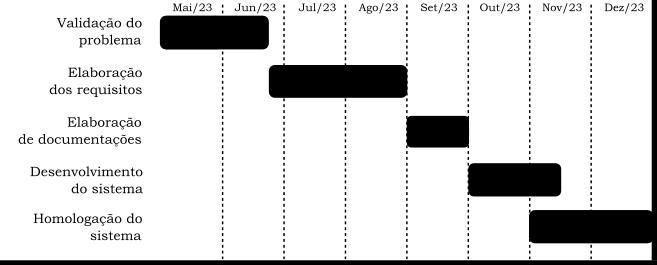
\includegraphics[width=260pt]{figuras/cronograma-atualizado}
    \caption{Cronograma atualizado do projeto}
    \label{fig-cronograma-atualizado}
    \end{center}
\end{figure}
  % -*- coding: utf-8; -*-

\chapter{Validação do problema}
\label{cha:validacao-problema}

A validação do problema foi efetuada por meio de entrevistas com alunos de graduação do Departamento de Informática. As entrevistas tinham como objetivo obter as opiniões de diferentes alunos em diferentes períodos de suas graduações quanto às suas preferências ao realizar as suas matrículas. As opiniões foram essenciais para planejar um algoritmo de recomendação que abrange as preferências do máximo de estudantes.

\section{Método das entrevistas}

Os entrevistados são alunos de graduação dos cursos do Departamento de Informática da PUC-Rio, cursando os cursos de engenharia da computação ou de ciência da computação. Foram selecionados vários alunos em diferentes estágios da graduação, do segundo ao sexto ano de graduação. Como algumas perguntas se referem às escolhas de disciplinas eletivas, e essas só começam a ser escolhidas no meio do período de graduação, não foram escolhidos estudantes no primeiro ano de graduação. 

\section{Perguntas realizadas}
A seguir estão as seis perguntas realizadas para cada entrevistado do Departamento de Informática, assim como uma explicação do motivo da pergunta ser realizada.

\begin{enumerate}
    \item \textbf{Qual é o seu curso e período atual?} O período atual do entrevistado é utilizado para entender o contexto de suas respostas, pois é necessário observar se o período em que o graduando está altera sua opinião ao realizar a sua matrícula. Como a quantidade de períodos propostos para a conclusão do curso variam de curso para curso no Departamento de Informática, também foi solicitado ao entrevistado seu curso para entender seu progresso de estudo na universidade e entender ainda melhor o contexto das suas próximas respostas.
        
        %% \textit{"Eu sou aluno de engenharia de computação, atualmente no sétimo período."}
    
    \item \textbf{Em média quantos créditos você faz num semestre?} A quantidade de créditos por semestre é relevante para que o algoritmo de recomendação tenha um conhecimento da média de disciplinas selecionadas por período. 
        %% \textit{"Nos últimos semestres eu tenho feito o limite máximo de 30 créditos, mas antes eu fazia uma média de 22 ou 24 créditos."}
    
    \item \textbf{Você se prepara com anteced\^encia para sua matr\'icula? Se sim, com quanta anteced\^encia? Se não, por quê?} Essa pergunta é fundamental para planejar uma expectativa de utilização da ferramenta de recomendação de disciplinas.
    
        %% \textit{"Sim, eu me prepararo assim que os horários das disciplinas são atualizados no microhorário. Normalmente dois dias antes da minha matrícula, eu já tenho algumas escolhas reservadas."}
    
    \item \textbf{Que crit\'erios você utiliza para escolher uma disciplina? Dados os critérios fornecidos, coloque-os em uma ordem de mais relevante para menos relevante.} Essa é a pergunta mais fundamental para o planejamento do algoritmo. Afinal, o objetivo do algoritmo de recomendação é recomendar disciplinas relevantes para um aluno. Por isso, é necessário saber o que torna uma disciplina relevante para ser escolhida.
        
        %% RESPOSTA INSERIDA NA PROXIMA SECÇÃO:
        %% \textit{"Eu acho que a matéria em si, se ela é mais difícil de entender ou mais fácil, e também o método de avaliação daquela disciplina, ou seja, se a nota final é composta de somente duas provas, ou se são vários pequenos trabalhos espalhados pelo semestre. Além disso, eu diria que o horário também é um limitador, porque não consigo ter aula sete da manhã todos os dias. Mas eu acho que o mais importante para mim é o professor: Se eu sei quem é o professor, sei que ele explica bem, vale a pena mesmo que a matéria seja mais difícil. Eu diria que a ordem dos critérios seria o professor, depois a matéria em si, depois o método de avaliação e por último o horário da disciplina."}

    \item \textbf{Como você procura disciplinas eletivas?} O objetivo dessa pergunta é descobrir como cada estudante procura as disciplinas eletivas, para saber quais são as principais fontes de informações utilizadas.
        
        %% \textit{"Eu normalmente procuro pela listagem completa das disciplinas do departamento, oferecida através do microhorário. Também havia uma lista de disciplinas eletivas oferecidas no próximo período que era enviada por email, mas esta nunca mais foi enviada ou atualizada."}

    \item \textbf{Você, pessoalmente, prefere disciplinas mais fáceis, mas que talvez não sejam muito úteis para a sua carreira, ou disciplinas mais relevantes mas que possam ser mais difíceis?} Essa pergunta pretende entender qual das duas opções é mais frequente. Caso a maioria dos estudantes preferem disciplinas mais fáceis, o algoritmo irá depender mais das notas dos alunos, e não tanto do conteúdo da disciplina em si. Caso a maioria dos estudantes preferem disciplinas mais relevantes, a nota pode não ser um valor tão relevante.
    
        %% RESPOSTA INSERIDA NA PROXIMA SECÇÃO:
        %% \textit{"Eu prefiro [disciplinas] eletivas mais fáceis, porque eu as vejo como uma oportunidade para facilitar a minha vida na faculdade, pois já tenho outras disciplinas mais difíceis para me preocupar. Eu encaro as [disciplinas] eletivas como um escape para poder respirar."}

\end{enumerate}

Ao final da entrevista, também foi oferecida a oportunidade de fornecer alguma opinião sobre o sistema de recomendação a ser desenvolvido.

\section{Resultados das entrevistas}

As seis perguntas foram separadas em três grupos, cada grupo com duas perguntas: \textit{Dados básicos dos estudantes} (perguntas 1 e 2), \textit{Escolha de disciplinas} (perguntas 3 e 4) e \textit{Disciplinas eletivas} (perguntas 5 e 6). A seguir estão os resultados das perguntas, separados pelos respectivos grupos.

\subsection{Dados básicos dos estudantes (Perguntas 1 e 2)}
\label{sec:dados-basicos-estudantes}

Dos onze entrevistados, cinco eram alunos de ciência de computação e os outros seis eram de engenharia de computação. cinco dos seis alunos entrevistados de engenharia de computação já haviam cursado mais da metade do curso (já cursaram 5 dos 10 semestres recomendados), e três dos cinco alunos entrevistados de ciência de computação já haviam cursado mais da metade do curso (já cursaram 4 dos 8 semestres recomendados). Além disso, dos onze alunos, nove eram homens e dois eram mulheres.

A distribuição dos períodos atuais dos entrevistados pode ser visualizada na figura \ref{fig:entrevista-grafico}. 

\begin{figure}[!ht]
    \begin{center}
    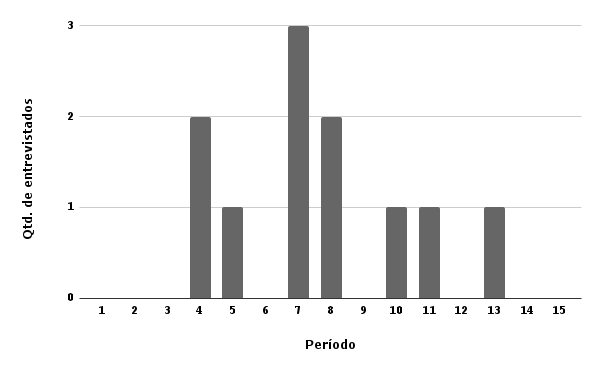
\includegraphics[width=350pt]{figuras/grafico-entrevista}
    \caption{Distribuição da quantidade de entrevistados pelos seus períodos atuais.}
    \label{fig:entrevista-grafico}
    \end{center}
  \end{figure}
  
A quantidade média de créditos por semestre dos alunos entrevistados é de 24 créditos, semelhante à quantidade média de créditos por semestre no currículo recomendado de ambos os cursos.

\subsection{Escolha de disciplinas (Perguntas 3 e 4)}
\label{sec:escolha-disciplinas}

Dez dos onze entrevistados se preparam com antecedência para a matrícula. Três desses utilizam como base o repositório de disciplinas microhorário para buscar as informações das disciplinas oferecidas para o pŕoximo período, e também utilizam o microhorário para descobrir quais são as disciplinas eletivas disponibilizadas no período. Todos os dez entrevistados utilizam o simulador de matrícula para confirmar suas escolhas. Apenas um dos entrevistados não se prepara com antecedência, fazendo suas pesquisas e escolhas durante o período da própria matrícula. 

Os critérios preferidos de cada aluno variam bastante. Por exemplo, um entrevistado citou que alguns critérios são  \textit{"a matéria em si, se ela é mais difícil de entender ou mais fácil, e também o método de avaliação, ou seja, se a nota final é composta de somente duas provas, ou se são vários trabalhos pequenos espalhados pelo semestre. Além disso, eu diria que o horário também é um limitador, porque não consigo ter aula sete da manhã todos os dias. Mas eu acho que o mais importante para mim é o professor: Se eu sei quem é o professor, sei que ele explica bem, vale a pena mesmo que a matéria seja mais difícil. Eu diria que a ordem dos critérios seria o professor, depois a matéria em si, depois o método de avaliação e por último o horário da disciplina."}.

Os critérios de escolha de disciplinas ditos nas entrevistas foram agrupados em cinco grupos: (1) Conteúdo da disciplina; (2) Professor; (3) Método de avaliação; (4) Horário da disciplina e (5) Opinião de amigos. A tabela \ref{tab:entrevista-criterios-raw} apresenta as respostas dos onze entrevistados e as suas respostas. O número indica em qual posição ficou aquele critério na ordem de preferência pessoal do aluno.

\begin{table}[!ht]
    \begin{center}
        \begin{tabular}{ l||c|c|c|c|c| } 
            & Conteúdo & Professor & Avaliação & Horário & Opinião \\ 
            \hline 
            \textit{Entrevistado 1 } & 3 & - & - & 1 & 2 \\     % miguel angelus
            \textit{Entrevistado 2 } & 1 & - & - & 3 & 2 \\     % joao biscaia
            \textit{Entrevistado 3 } & 2 & 3 & - & - & 1 \\     % laura luz 
            \textit{Entrevistado 4 } & 3 & 1 & - & 2 & - \\     % thomas botelho
            \textit{Entrevistado 5 } & 2 & - & - & 1 & 3 \\     % rafael lavatori
            \textit{Entrevistado 6 } & 1 & - & - & - & - \\     % antenor bastos
            \textit{Entrevistado 7 } & 1 & - & - & - & - \\     % jeronimo soares
            \textit{Entrevistado 8 } & 2 & 3 & 1 & 4 & - \\     % mariana barreto
            \textit{Entrevistado 9 } & 3 & 2 & - & - & 1 \\     % paulo de tarso
            \textit{Entrevistado 10} & 1 & - & 3 & 2 & - \\     % luiz fellipe
            \textit{Entrevistado 11} & - & 2 & - & 1 & - \\     % miguel
        \end{tabular}
    \end{center}
    \caption{Graus dos critérios de escolhas de disciplinas escolhidos pelos 
    entrevistados}
    % O número indica o grau de importância, onde 1 é o mais importante. Os critérios sem números são critérios não citados pelo entrevistado na entrevista.
    
    \label{tab:entrevista-criterios-raw}
\end{table}

Para gerar uma comparação dos critérios, foi dado um peso para cada grau de importância. Quanto maior o grau de importância. A tabela \ref{tab:grau-peso} exibe a relação entre os graus de importância e os pesos. 

\begin{table}[!ht]
    \begin{center}
        \begin{tabular}{ r||c|c|c|c|c| } 
            \textit{Grau} & 1 & 2 & 3 & 4 & - \\
            \hline 
            \textit{Peso} & 5 & 4 & 3 & 2 & 0 \\
        \end{tabular}
    \end{center}
    \caption{Relação de peso para grau dos critérios de escolhas}
    \label{tab:grau-peso}
\end{table}

Ao substituir os pesos da Tabela \ref{tab:grau-peso} na Tabela \ref{tab:entrevista-criterios-raw}, é possível somar os pesos para cada critério de escolha e obter uma relação entre eles, conforme a tabela \ref{tab:entrevista-criterios-peso}.

\begin{table}[!ht]
    \begin{center}
        \begin{tabular}{ l||c|c|c|c|c| } 
            & Conteúdo & Professor & Avaliação & Horário & Opinião \\ 
            \hline 
            \textit{Entrevistado 1 } & 3 & 0 & 0 & 5 & 4 \\     % miguel angelus
            \textit{Entrevistado 2 } & 5 & 0 & 0 & 3 & 4 \\     % joao biscaia
            \textit{Entrevistado 3 } & 4 & 3 & 0 & 0 & 5 \\     % laura luz 
            \textit{Entrevistado 4 } & 3 & 5 & 0 & 4 & 0 \\     % thomas botelho
            \textit{Entrevistado 5 } & 4 & 0 & 0 & 5 & 3 \\     % rafael lavatori
            \textit{Entrevistado 6 } & 5 & 0 & 0 & 0 & 0 \\     % antenor bastos
            \textit{Entrevistado 7 } & 5 & 0 & 0 & 0 & 0 \\     % jeronimo soares
            \textit{Entrevistado 8 } & 4 & 3 & 5 & 2 & 0 \\     % mariana barreto
            \textit{Entrevistado 9 } & 3 & 4 & 0 & 0 & 5 \\     % paulo de tarso
            \textit{Entrevistado 10} & 5 & 0 & 3 & 4 & 0 \\     % luiz fellipe
            \textit{Entrevistado 11} & 0 & 4 & 0 & 5 & 0 \\     % miguel
            \hline
            \textbf{Soma}            & 41& 19& 8 & 28& 21 
        \end{tabular}
    \end{center}
    \caption{Pesos dos critérios de escolhas de disciplinas escolhidos pelos entrevistados.}
    %  O número indica o valor relativo ao grau de importância, onde 5 é o mais importante.
    \label{tab:entrevista-criterios-peso}
\end{table}

Observando a Tabela \ref{tab:entrevista-criterios-peso}, as somas dos pesos indicam que a ordem dos critérios mais relevantes na escolha de uma disciplina, do mais relevante para o menos relevante:
\textit{Conteúdo da disciplina}, \textit{Horário da disciplina}, \textit{Opinião de amigos}, \textit{Professor} e \textit{Método de avaliação}.

\subsection{Disciplinas eletivas (Perguntas 5 e 6)}
\label{sec:disciplinas-eletivas}

Dos onze entrevistados, nove citaram a utilização do microhorário para coletar as disciplinas eletivas do período. Os outros dois dependem mais de recomendação de amigos. Três entrevistados procuram por uma listagem oficial de disciplinas eletivas oferecidas pelo departamento para o próximo período, mas nem sempre encontram essa listagem oficial.

Por último, quatro entrevistados preferem disciplinas eletivas mais fáceis, enquanto três entrevistados preferem disciplinas eletivas que sejam mais relevantes para a sua formação. Os quatro restantes preferem um equilíbrio entre facilidade e relevância. Dois entrevistados disseram que inicialmente escolhem disciplinas mais relevantes, mas que ao decorrer dos períodos optam por eletivas mais fáceis. Uma das respostas foi que \textit{"[Eu] prefiro [disciplinas] eletivas mais fáceis, porque eu as vejo como uma oportunidade para facilitar a minha vida na faculdade, pois já tenho outras disciplinas mais difíceis para me preocupar. Eu encaro as [disciplinas] eletivas como um escape para poder respirar."}

  % -*- coding: utf-8; -*-

\chapter{Requisitos}
\label{cha:Requisitos}

Os requisitos estão divididos em requisitos relacionados ao sistema e requisitos relacionados ao algoritmo.
Os requisitos do sistema dizem respeito ao sistema que disponibiliza o serviço de montagem de grade horária do próximo período, assim como um serviço de avaliar disciplinas e professores, que existe para satisfazer as necessidades observadas nos capítulos anteriores. Os requisitos do algoritmo dizem respeito às entradas e saídas do algoritmo afim de se produzir uma recomendação adequada de acordo as necessidades observadas no capítulo \ref{cha:validacao-problema}.

\section{Do algoritmo}

Os requisitos do algoritmo de recomendação de disciplinas precisam satisfazer os critérios de escolha de disciplinas mais relevantes, discutidos no capítulo \ref{sec:escolha-disciplinas}, ou seja, recomendar de acordo com o conteúdo da disciplina, horários disponíveis, opiniões de amigos, o professor, e por último o método de avaliação.
Além disso, para satisfazer a preferência de disciplinas eletivas discutidas no capítulo \ref{sec:disciplinas-eletivas}, os requisitos precisam satisfazer a preferência de recomendar disciplinas com base na sua facilidade.

A lista de requisitos do algoritmo está disponível na tabela \ref{tab:req-algoritmo}.

\begin{table}[!ht]
    \begin{center}
        \begin{tabular}{ | m{0.1\textwidth} | p{0.8\textwidth} | }  
            \hline
            \textbf{RF01} & O algoritmo deve receber as disciplinas e turmas oferecidas no próximo semestre conforme o microhorário.\tabularnewline\hline
            \textbf{RF02} & O algoritmo deve receber opcionalmente a grade curricular do curso que o aluno está cursando.\tabularnewline\hline
            \textbf{RF03} & O algoritmo deve receber as avaliações das disciplinas e professores fornecidas pelos usuários do sistema.\tabularnewline\hline
            \textbf{RF04} & O algoritmo deve receber opcionalmente o histórico escolar do aluno.\tabularnewline\hline
            \textbf{RF05} & O algoritmo deve receber disciplinas já selecionadas pelo aluno.\tabularnewline\hline
            \textbf{RF06} & O algoritmo deve retornar recomendações de disciplinas com base nas entradas fornecidas.\tabularnewline\hline
            
            \textbf{RNF1} & O algoritmo deve retornar as recomendações em menos de 3 segundos.\tabularnewline\hline
            \textbf{RNF2} & O algoritmo deve ser determinístico, ou seja, retorna as mesmas recomendações para as mesmas entradas.\tabularnewline\hline
        \end{tabular}
    \end{center}
    \caption{Requisitos do algoritmo}
    
    \label{tab:req-algoritmo}
\end{table}

\section{Do sistema}

O sistema precisa satisfazer as necessidades do usuário e também as necessidades do algoritmo, pois o sistema hospeda o algoritmo de recomendação.
Os requisitos do sistema estão disponíveis na tabela \ref{tab:req-sistema}.

\begin{table}[!ht]
    \begin{center}
        \begin{tabular}{ | m{0.1\textwidth} | p{0.8\textwidth} | }  
            \hline
            \textbf{RF07} & O sistema deve permitir que o usuário crie uma grade horária para o próximo período.\tabularnewline\hline
            \textbf{RF08} & O sistema deve permitir que o usuário submita seu histórico escolar.\tabularnewline\hline
            \textbf{RF09} & O sistema deve permitir que o usuário selecione turmas das disciplinas para compor sua grade horária.\tabularnewline\hline
            \textbf{RF10} & O sistema deve permitir que o usuário autenticado armazene a sua grade horária finalizada.\tabularnewline\hline
            \textbf{RF11} & O sistema deve permitir que o usuário compartilhe a sua grade horária finalizada. \tabularnewline\hline
            \textbf{RF12} & O sistema deve permitir que o usuário recupere uma grade horária montada a partir de um link compartilhado.\tabularnewline\hline
            
            \textbf{RF13} & O sistema deve permitir que o usuário inicie uma sessão autenticada.\tabularnewline\hline
            \textbf{RF14} & O sistema deve permitir que o usuário finalize uma sessão autenticada.\tabularnewline\hline
            \textbf{RF15} & O sistema deve permitir que o usuário autenticado avalie uma disciplina.\tabularnewline\hline
            \textbf{RF16} & O sistema deve permitir que o usuário autenticado avalie um professor de uma disciplina.\tabularnewline\hline
            \textbf{RF17} & O sistema deve permitir que o usuário autenticado altere uma avaliação feita anteriormente.\tabularnewline\hline

            \textbf{RF18} & O sistema deve periodiacamente sincronizar as vagas e turmas com o microhorário.\tabularnewline\hline
            \textbf{RF19} & O sistema deve periodiacamente adicionar novas disciplinas conforme disponibilizado no microhorário.\tabularnewline\hline

            %% \textbf{RNF3} & O sistema deve estar disponível publicamente aos alunos da universidade.\tabularnewline\hline
            \textbf{RNF3} & O sistema deve suportar pelo menos 40 usuários simultâneos.\tabularnewline\hline
        
        \end{tabular}
    \end{center}
    \caption{Requisitos do sistema}
    
    \label{tab:req-sistema}
\end{table}

  % -*- coding: utf-8; -*-

%% https://linorg.usp.br/CTAN/macros/latex/required/tools/longtable.pdf %%
%% http://ctan.dcc.uchile.cl/macros/latex/required/tools/longtable.pdf %%

\chapter{Casos de Uso}
\label{cha:Casos de Uso}

Os casos de uso do sistema servem para descrever como o sistema pode ser utilizado afim de se satisfazer as necessidades do usuário.
Os casos de uso referenciam os requisitos do sistema descritos no capítulo \ref{cha:Requisitos}.
A figura \ref{fig:diagrama-casos-uso} contém o diagrama de casos de uso do sistema.

\begin{figure}[ht]
    \begin{center}
    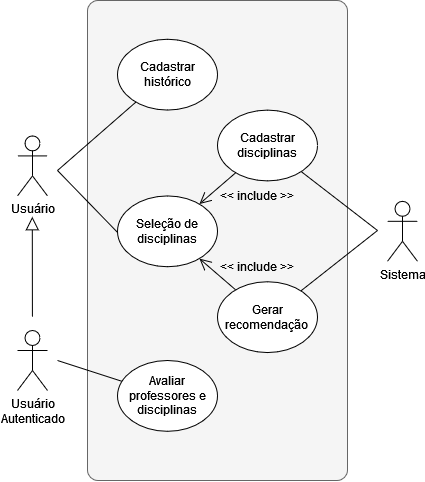
\includegraphics[width=250pt]{figuras/casos-uso.png}
    \caption{Diagrama dos casos de uso}
    \label{fig:diagrama-casos-uso}
    \end{center}
\end{figure}

A seguir estão as descrições dos casos de uso presentes na figura \ref{fig:diagrama-casos-uso}.

\begin{longtable}{ | m{0.3\textwidth} | m{0.7\textwidth} | }
    \hline\hline
    \multicolumn{2}{|c|}{Caso de Uso \textbf{UC01} - Cadastrar disciplinas}\tabularnewline\hline\hline\endfirsthead
    \hline\hline
    \multicolumn{2}{|c|}{Caso de Uso \textbf{UC01} (continuação)}\tabularnewline\hline\hline\endhead
    \hline\endfoot
    \hline\caption{Caso de uso UC01}\endlastfoot

    \textbf{Objetivo} & Permitir que o sistema atualize as disciplinas no seu banco de dados, incluindo as eletivas.\tabularnewline\hline 
    \textbf{Requisitos} & RF01 e RF10\tabularnewline\hline
    \textbf{Atores} & Sistema\tabularnewline\hline
    \textbf{Pré condições} & Não se aplica\tabularnewline\hline

    \multirow{1}{*}{\textbf{Fluxo principal}} & [1] O sistema acessa o microhorário, coletando informações de todas as disciplinas.\tabularnewline\cline{2-2}
    & [2] O sistema trata e converte as informações para o modelo do banco.\textbf{[A1]}\tabularnewline\cline{2-2}
    & [3] O sistema cria uma nova versão do banco, com as novas informações.\tabularnewline\cline{2-2}
    & [4] O sistema remove a versão antiga do banco caso o passo 3 tenha sido executado com sucesso.\tabularnewline\cline{2-2}
    & [5] O sistema atualiza a data e hora da última atualização do microhorário que aparece na interface.\tabularnewline\cline{2-2}
    & [6] O caso de uso é encerrado.
    \label{tab:uc01}
\end{longtable}


\begin{longtable}{ | m{0.3\textwidth} | m{0.7\textwidth} | }
    
    \hline\hline    
    \multicolumn{2}{|c|}{Caso de Uso \textbf{UC02} - Cadastrar histórico}\tabularnewline\hline\hline\endfirsthead
    \hline\hline
    \multicolumn{2}{|c|}{Caso de Uso \textbf{UC02} (continuação)}\tabularnewline\hline\hline\endhead
    \hline\endfoot
    \hline\caption{Caso de uso UC02}\endlastfoot

    \textbf{Objetivo} & Permitir que o usuário cadastre seu histórico escolar ou outras informações no sistema para personalizar as recomendações.\tabularnewline\hline
    \textbf{Requisitos} & RF02, RF04, RF08 e RF09\tabularnewline\hline
    \textbf{Atores} & Usuário\tabularnewline\hline
    \textbf{Pré condições} & O usuário seleciona a opção "Montar Grade Horária", e este não possui nenhuma informação pré-cadastrada.\tabularnewline\hline

    \multirow{1}{*}{\textbf{Fluxo principal}} & [1] O sistema exibe uma tela solicitando o histórico escolar do aluno, e um botão de pular.\tabularnewline\cline{2-2}
    & [2] O usuário submete o histórico escolar. \textbf{[A1]}\tabularnewline\cline{2-2}
    & [3] O sistema armazena o histórico, curso atual, período atual e o currículo do aluno.\tabularnewline\cline{2-2}
    & [4] O sistema exibe a tela de criação de grade horária.\tabularnewline\cline{2-2}
    & [5] O caso de uso é encerrado.\tabularnewline\hline

    \multirow{1}{*}{\textbf{Fluxos Alternativos}} & \textbf{[A1] O usuário pressiona o botão de pular}\tabularnewline\cline{2-2}
    & [1] O sistema exibe uma tela solicitando o curso atual, período atual, o currículo do aluno, um botão de pular e um botão de continuar.\tabularnewline\cline{2-2}
    & [2] O usuário preenche o formulário e pressiona o botão de continuar. \textbf{[A2]}\tabularnewline\cline{2-2} 
    & [3] O sistema armazena as informações fornecidas.\tabularnewline\cline{2-2}
    & [4] O sistema exibe a tela de criação de grade horária.\tabularnewline\cline{2-2}
    & [5] O caso de uso é encerrado.\tabularnewline\cline{2-2}

    & \textbf{[A2] O usuário pressiona o botão de pular}\tabularnewline\cline{2-2}
    & [1] O sistema altera o funcionamento para recomendações genéricas.\tabularnewline\cline{2-2}
    & [2] O sistema exibe a tela de criação de grade horária. \textbf{[A2]}\tabularnewline\cline{2-2} 
    & [3] O caso de uso é encerrado. %% \tabularnewline\cline{2-2}
    \label{tab:uc02}
\end{longtable}


\begin{longtable}{ | m{0.3\textwidth} | m{0.7\textwidth} | }
    \hline\hline
    \multicolumn{2}{|c|}{Caso de Uso \textbf{UC03} - Gerar recomendações}\tabularnewline\hline\hline\endfirsthead
    \hline\hline
    \multicolumn{2}{|c|}{Caso de Uso \textbf{UC03} (continuação)}\tabularnewline\hline\hline\endhead
    \hline\endfoot
    \hline\caption{Caso de uso UC03}\endlastfoot

    \textbf{Objetivo} & Permitir que o sistema recomende disciplinas para o usuário.\tabularnewline\hline 
    \textbf{Requisitos} & RF01-06\tabularnewline\hline
    \textbf{Atores} & Sistema\tabularnewline\hline
    \textbf{Pré condições} & O usuário deve ter modificado a grade horária.\tabularnewline\hline

    \multirow{1}{*}{\textbf{Fluxo principal}} & [1] O sistema coleta as disciplinas e turmas já adicionadas no grade horária do usuário.\tabularnewline\cline{2-2}
    & [2] O sistema recupera o histórico escolar do usuário do banco de dados, caso o usuário tenha submetido.\textbf{[A1]}\tabularnewline\cline{2-2}
    & [3] O sistema utiliza o algoritmo para gerar recomendações de disciplinas para o usuário.\tabularnewline\cline{2-2}
    & [4] O sistema exibe as recomendações na interface do usuário\tabularnewline\cline{2-2}
    & [5] O caso de uso é encerrado.
    \label{tab:uc03}
\end{longtable}


\begin{longtable}{ | m{0.3\textwidth} | m{0.7\textwidth} | }
    
    \hline\hline
    \multicolumn{2}{|c|}{Caso de Uso \textbf{UC04} - Selecionar disciplina}\tabularnewline\hline\hline\endfirsthead
    \hline\hline
    \multicolumn{2}{|c|}{Caso de Uso \textbf{UC04} (continuação)}\tabularnewline\hline\hline\endhead
    \hline\endfoot
    \hline\caption{Caso de uso UC04}\endlastfoot

    \textbf{Objetivo} & Permitir que o usuário adicione e remova disciplinas da sua grade.\tabularnewline\hline
    \textbf{Requisitos} & RF1\tabularnewline\hline
    \textbf{Atores} & Usuário\tabularnewline\hline
    \textbf{Pré condições} & O usuário está na área de criação da grade horária.\tabularnewline\hline

    \multirow{1}{*}{\textbf{Fluxo principal}} & [1] O sistema exibe a grade horária do usuário, uma lista de disciplinas disponíveis, uma lista de disciplinas recomendadas e um campo de texto para pesquisa.\tabularnewline\cline{2-2}
    & [2] O usuário seleciona uma disciplina da lista de disciplinas disponíveis ou recomendadas. \textbf{[A1]} \textbf{[A2]} .\tabularnewline\cline{2-2}
    & [3] O sistema exibe as turmas disponíveis para a disciplina selecionada e um botão de voltar.\tabularnewline\cline{2-2}
    & [4] O usuário seleciona uma das turmas exibidas. \textbf{[A3]}\tabularnewline\cline{2-2}
    & [5] O sistema acrescenta a turma selecionada na grade horária, e recalcula as disciplinas recomendadas. \tabularnewline\cline{2-2}
    & [6] O caso de uso é encerrado.\tabularnewline\hline

    \multirow{1}{*}{\textbf{Fluxos Alternativos}} & \textbf{[A1] O sistema seleciona uma das disciplinas na sua grade horária}\tabularnewline\cline{2-2}
    & [1] O sistema exibe informações da disciplina e turma selecionada, um botão de voltar e um botão de excluir.\tabularnewline\cline{2-2} 
    & [2] O usuário seleciona o botão de excluir. \textbf{[A3]}\tabularnewline\cline{2-2} 
    & [3] O sistema remove a turma e disciplina da grade horária do usuário, e recalcula as disciplinas recomendadas. \tabularnewline\cline{2-2}
    & [4] O sistema volta para o passo 1 do fluxo principal. \tabularnewline\cline{2-2}

    & \textbf{[A2] O usuário preenche o campo de texto para pesquisa}\tabularnewline\cline{2-2}
    & [1] O sistema altera a lista de disciplinas, filtrando de acordo com o texto do campo de pesquisa. \tabularnewline\cline{2-2}
    & [2] O sistema volta para o passo 1 do fluxo principal. \tabularnewline\cline{2-2}

    & \textbf{[A3] O usuário pressiona o botão de voltar}\tabularnewline\cline{2-2}
    & [1] O sistema volta para o passo 1 do fluxo principal. %% \tabularnewline\cline{2-2}

    \label{tab:uc04}
\end{longtable}


\begin{longtable}{ | m{0.3\textwidth} | m{0.7\textwidth} | }
    \hline\hline
    \multicolumn{2}{|c|}{Caso de Uso \textbf{UC05} - Avaliar disciplinas e professores}\tabularnewline\hline\hline\endfirsthead
    \hline\hline
    \multicolumn{2}{|c|}{Caso de Uso \textbf{UC05} (continuação)}\tabularnewline\hline\hline\endhead
    \hline\endfoot
    \hline\caption{Caso de uso UC05}\endlastfoot

    \textbf{Objetivo} & Permitir que o usuário avalie uma disciplina ou um professor.\tabularnewline\hline
    \textbf{Requisitos} & RF03, RF16 e RF17\tabularnewline\hline
    \textbf{Atores} & Usuário\tabularnewline\hline
    \textbf{Pré condições} & Não se aplica.\tabularnewline\hline

    \multirow{1}{*}{\textbf{Fluxo principal}} & [1] O sistema exibe uma lista de disciplinas e professores e um campo de texto para pesquisa.\tabularnewline\cline{2-2}
    & [2] O usuário seleciona uma disciplina. \textbf{[A1]} \textbf{[A2]}\tabularnewline\cline{2-2}
    & [3] O sistema exibe uma tela para avaliar a disciplina em conteúdo e dificuldade, um botão de salvar e um botão de voltar.\tabularnewline\cline{2-2}
    & [4] O usuário avalia a disciplina e seleciona o botão de salvar. \textbf{[A3]}\tabularnewline\cline{2-2}
    & [5] O sistema armazena a avaliação do usuário.\tabularnewline\cline{2-2}
    & [6] O caso de uso é encerrado.\tabularnewline\hline

    \multirow{1}{*}{\textbf{Fluxos Alternativos}} & \textbf{[A1] O usuário seleciona um professor}\tabularnewline\cline{2-2}
    & [1] O sistema exibe uma tela para avaliar o professor, um botão de salvar e um botão de voltar.\tabularnewline\cline{2-2}
    & [2] O usuário avalia o professor e seleciona o botão de salvar. \textbf{[A3]}\tabularnewline\cline{2-2} 
    & [3] O sistema armazena a avaliação do usuário.\tabularnewline\cline{2-2}
    & [4] O caso de uso é encerrado.\tabularnewline\cline{2-2}

    & \textbf{[A2] O usuário preenche o campo de texto para pesquisa}\tabularnewline\cline{2-2}
    & [1] O sistema exibe disciplinas e professores utilizando como filtro o texto do usuário.\tabularnewline\cline{2-2}
    & [2] O sistema volta para o passo 1 do fluxo principal.\tabularnewline\cline{2-2}

    & \textbf{[A2] O usuário seleciona o botão de voltar}\tabularnewline\cline{2-2}
    & [2] O sistema volta para o passo 1 do fluxo principal. %%\tabularnewline\cline{2-2} 

    \label{tab:uc05}
\end{longtable}

Para melhor descrever a interação do usuário com o sistema com a interface da criação de grade horária e com o algoritmo de recomendação, a figura \ref{fig:fluxograma-grade} apresenta um fluxograma com as possíveis ações do usuário na interface. Neste diagrama, os retângulos representam componentes da interface passíveis de interação do usuário, os hexágonos representam operações efetuadas pelo sistema, e o losango representa uma tomada de decisão pelo sistema. Além disso, as setas contínuas representam operações do usuário, e as setas tracejadas representam transições automáticas entre os componentes e operações. 

\begin{figure}[ht]
    \begin{center}
    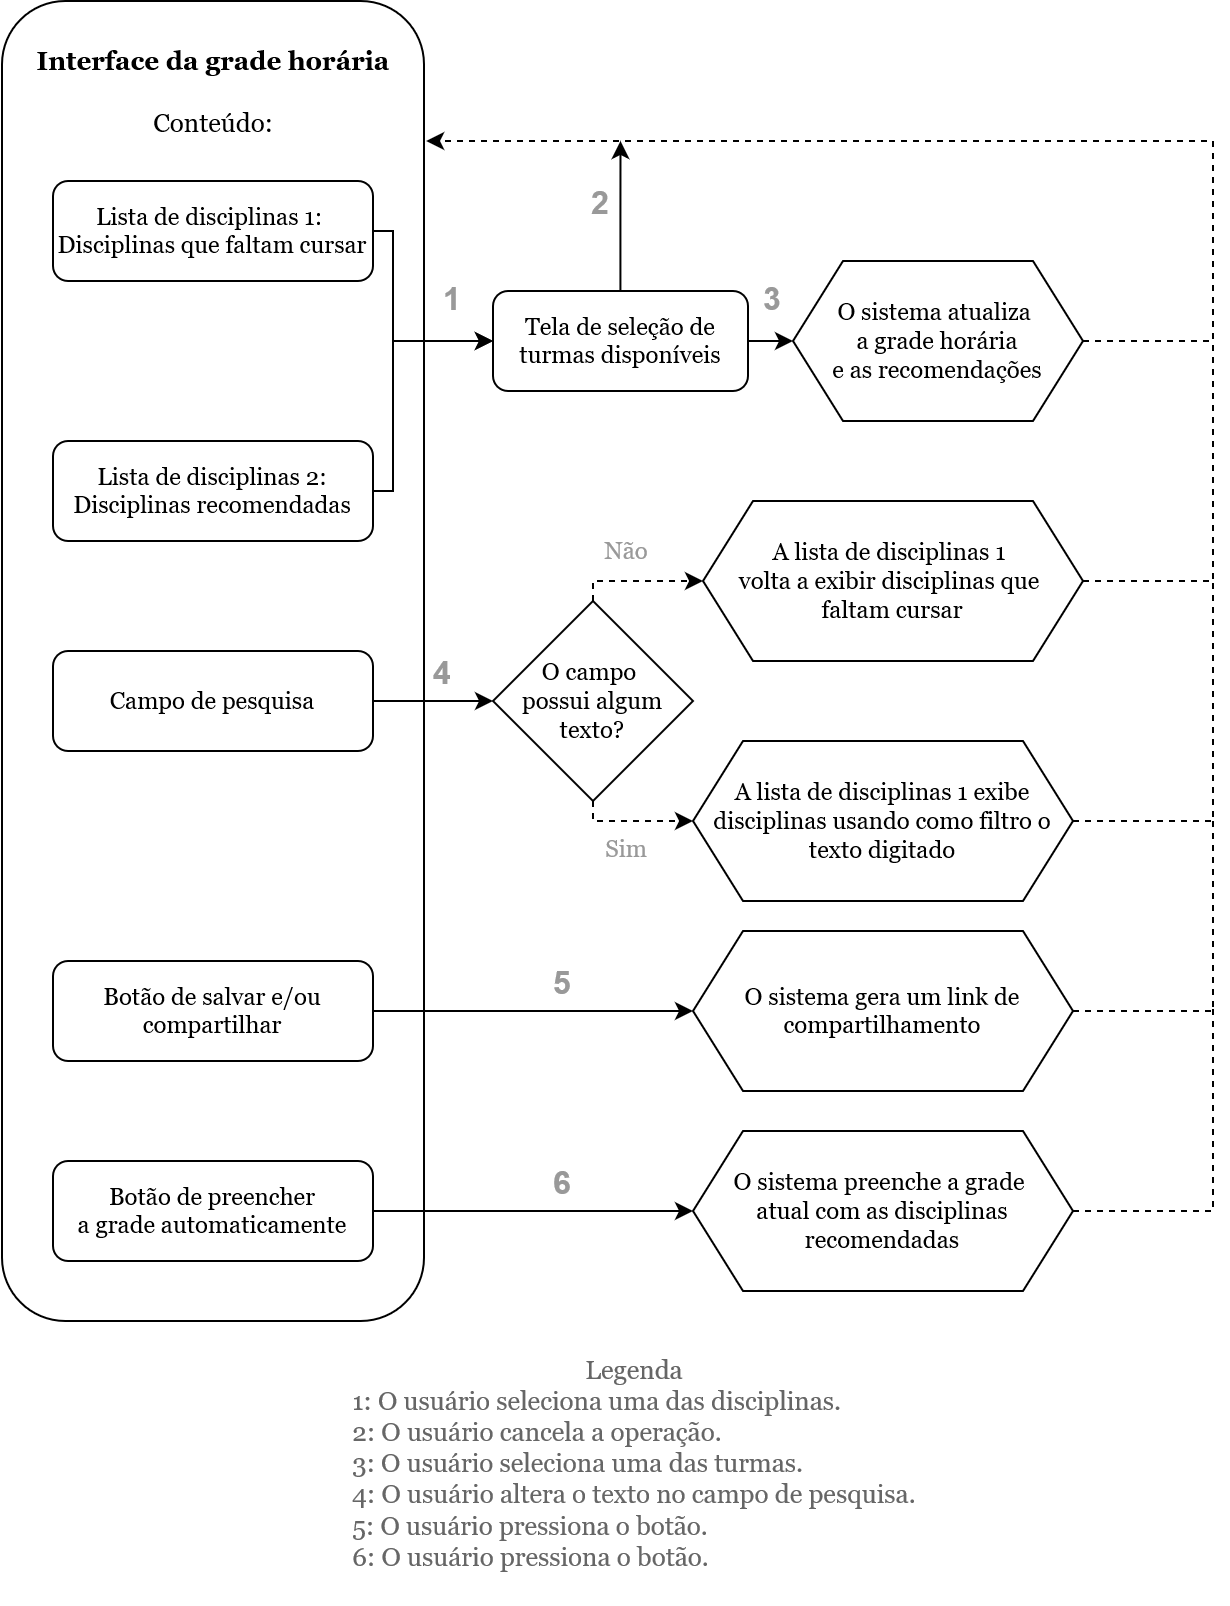
\includegraphics[width=390pt]{figuras/fluxograma-grade.drawio.png}
    \caption{Fluxograma da interface de criação de grade horária}
    \label{fig:fluxograma-grade}
    \end{center}
\end{figure}
  \chapter{Wireframe}
\label{cha:Wireframe}

Um \textit{wireframe} é um protótipo da interface do sistema, que serve para ilustrar o funcionamento e interação do usuário com o sistema. A seguir estão três telas do sistema: a página inicial, a página de criação de grade horária, e a página de avaliação de disciplinas. Essas são as principais páginas do sistema.

\begin{figure}[ht]
    \begin{center}
    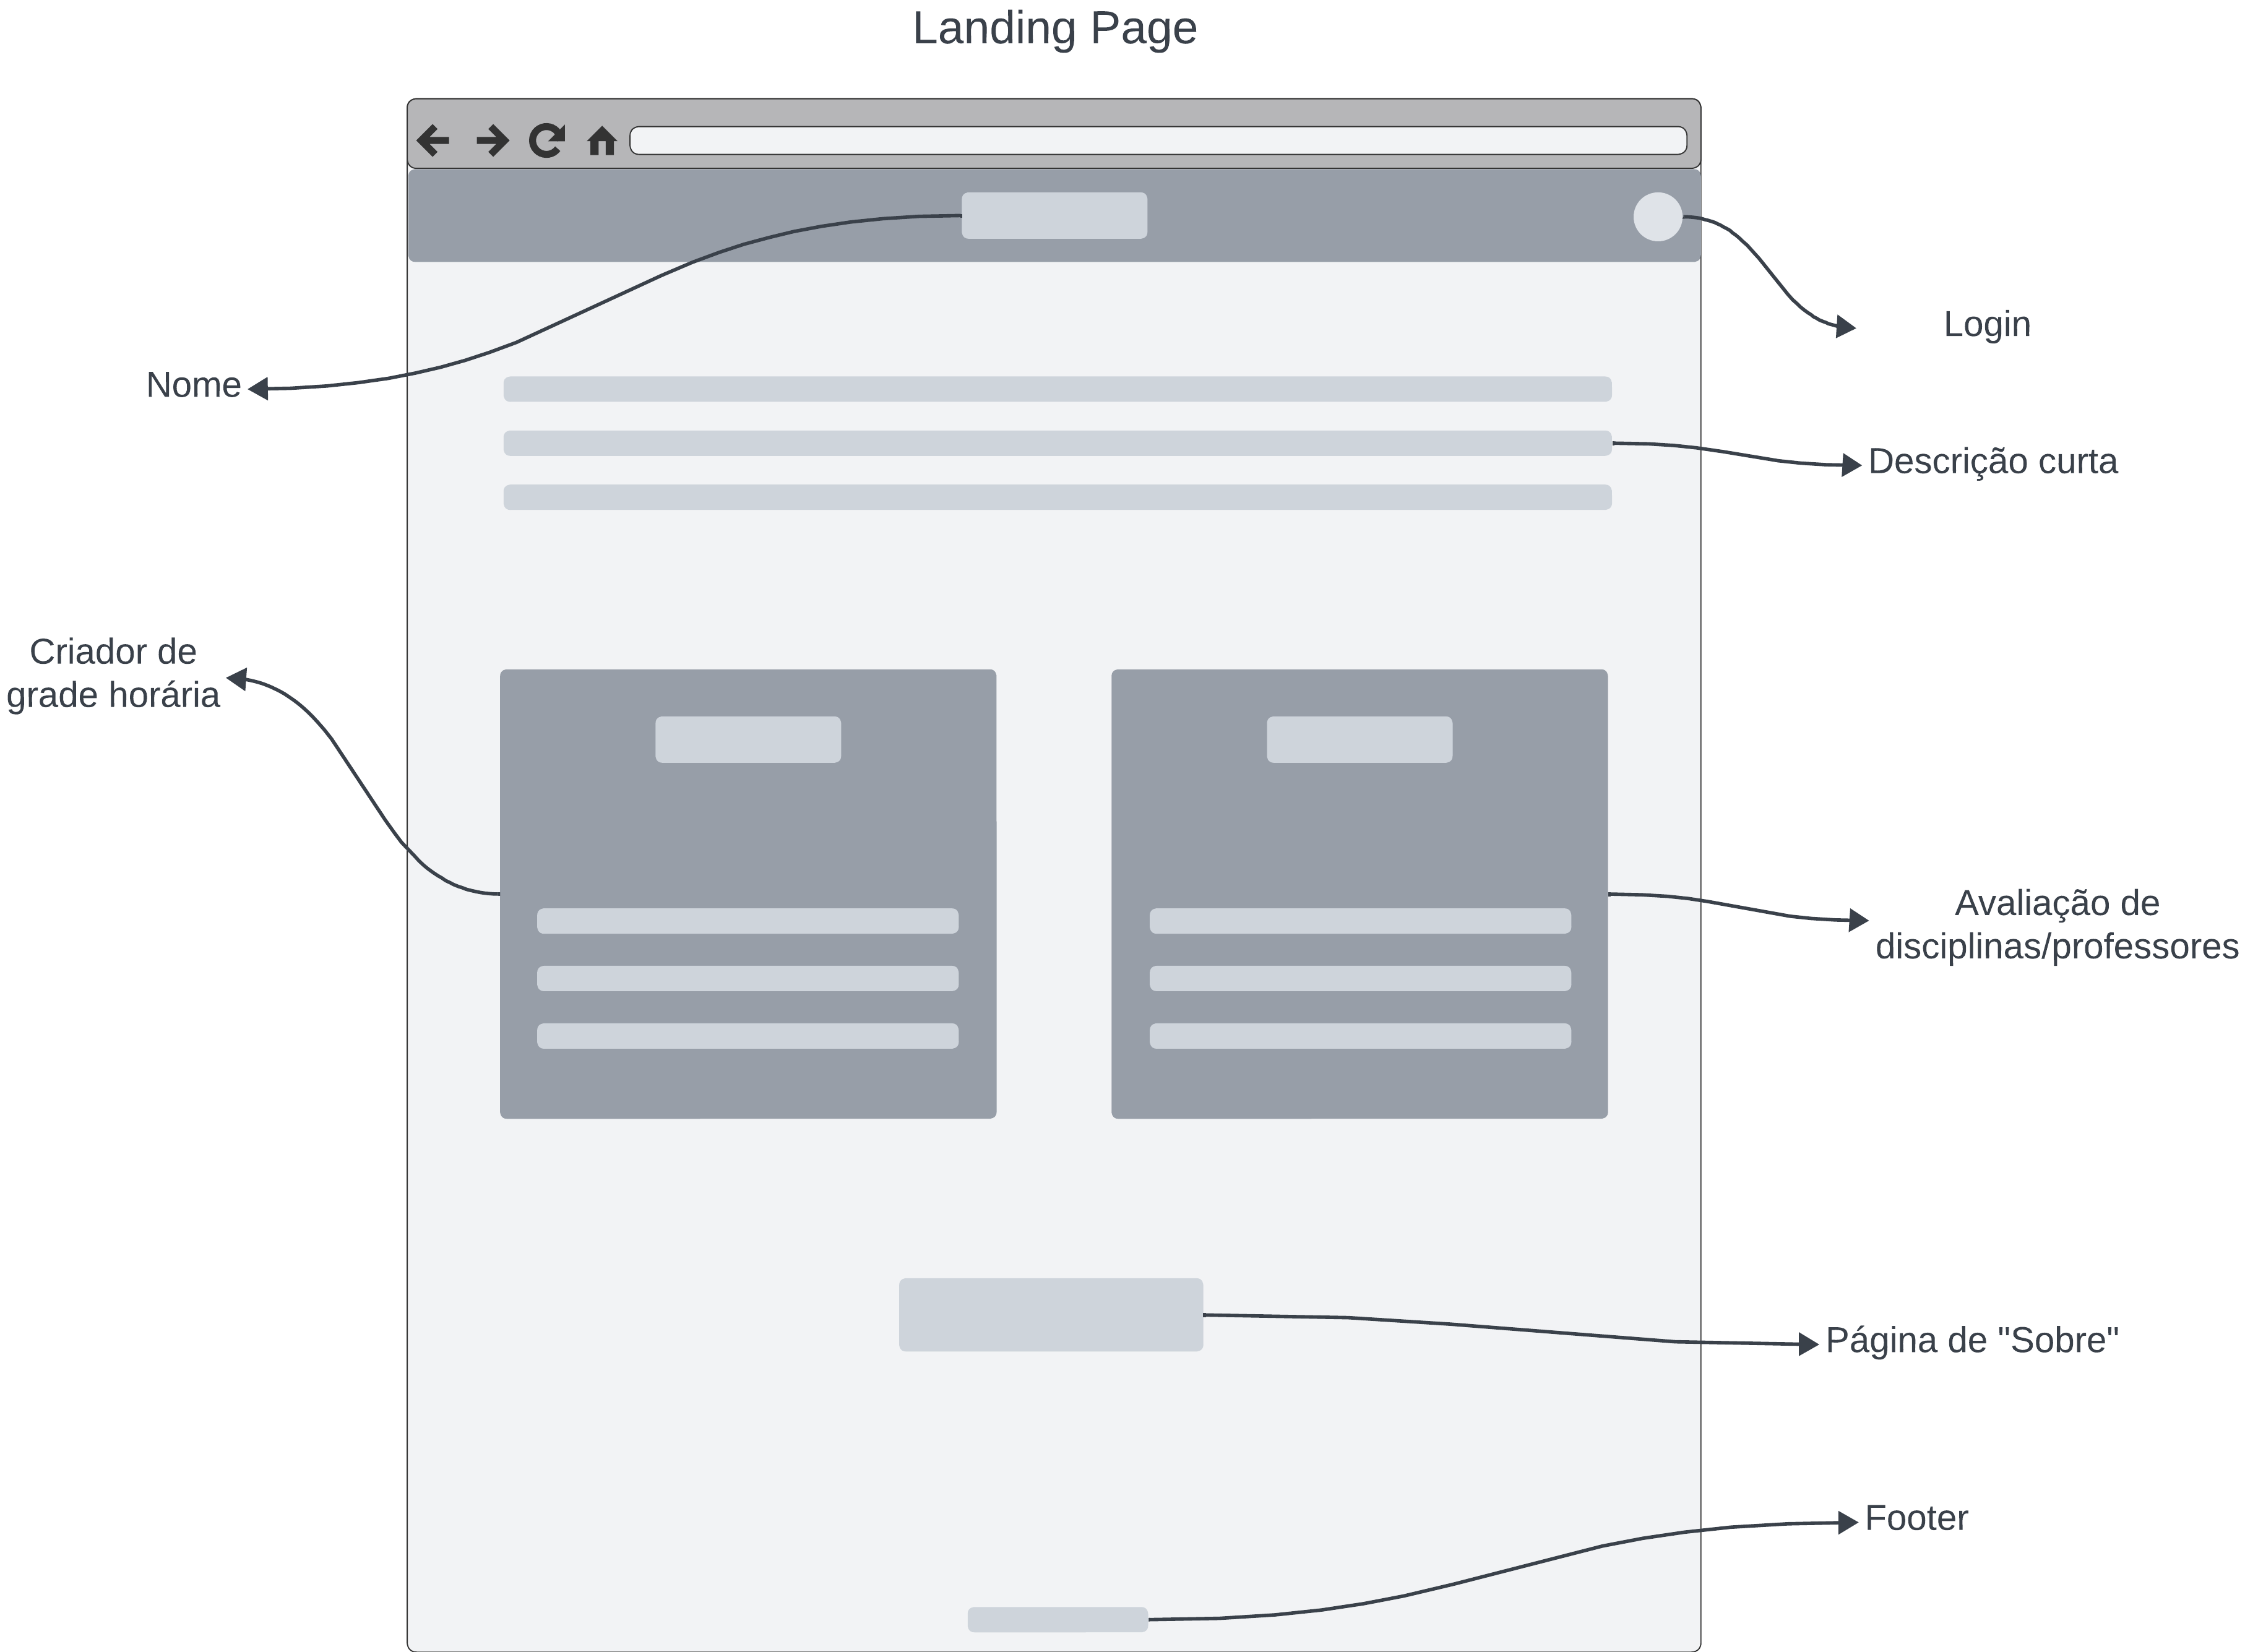
\includegraphics[width=390pt]{figuras/pagina-inicial.png}
    \caption{Wireframe da página inicial (\textit{Landing Page})}
    \label{fig:wireframe-pagina-inicial}
    \end{center}
\end{figure}

\begin{figure}[ht]
    \begin{center}
    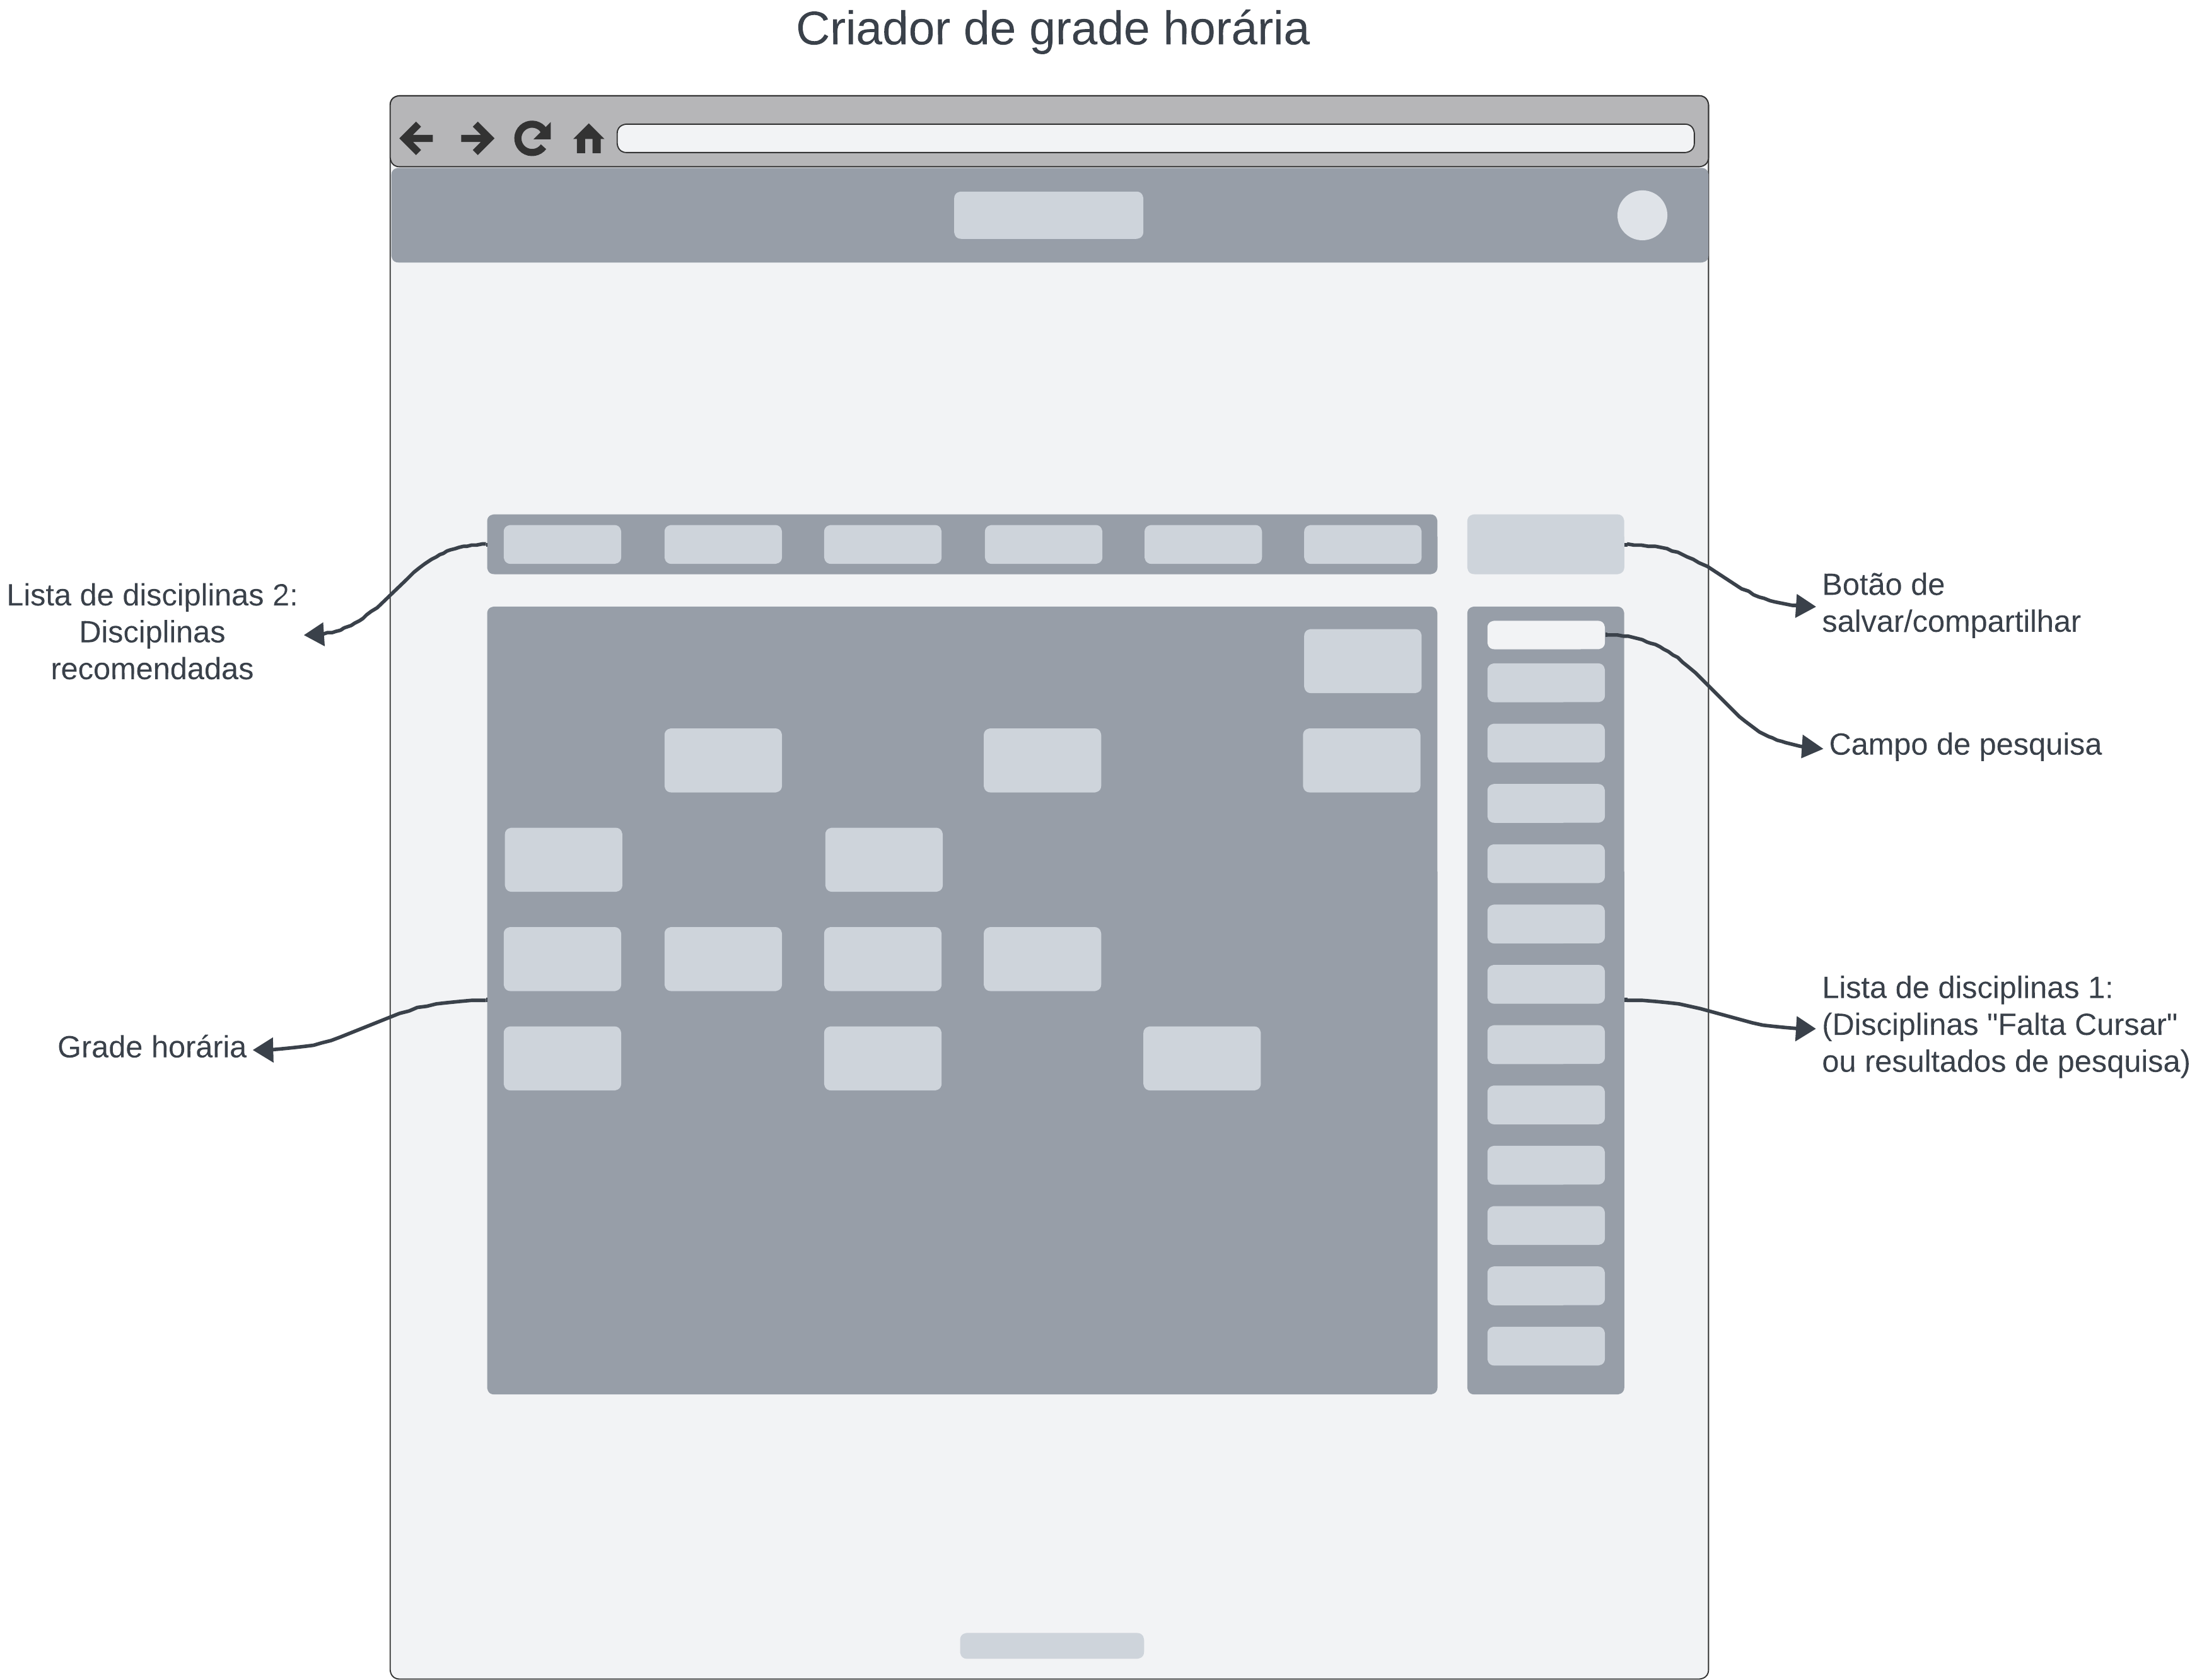
\includegraphics[width=390pt]{figuras/pagina-criacao.png}
    \caption{Wireframe da página de criação de grade horária}
    \label{fig:wireframe-pagina-criacao}
    \end{center}
\end{figure}

\begin{figure}[ht]
    \begin{center}
    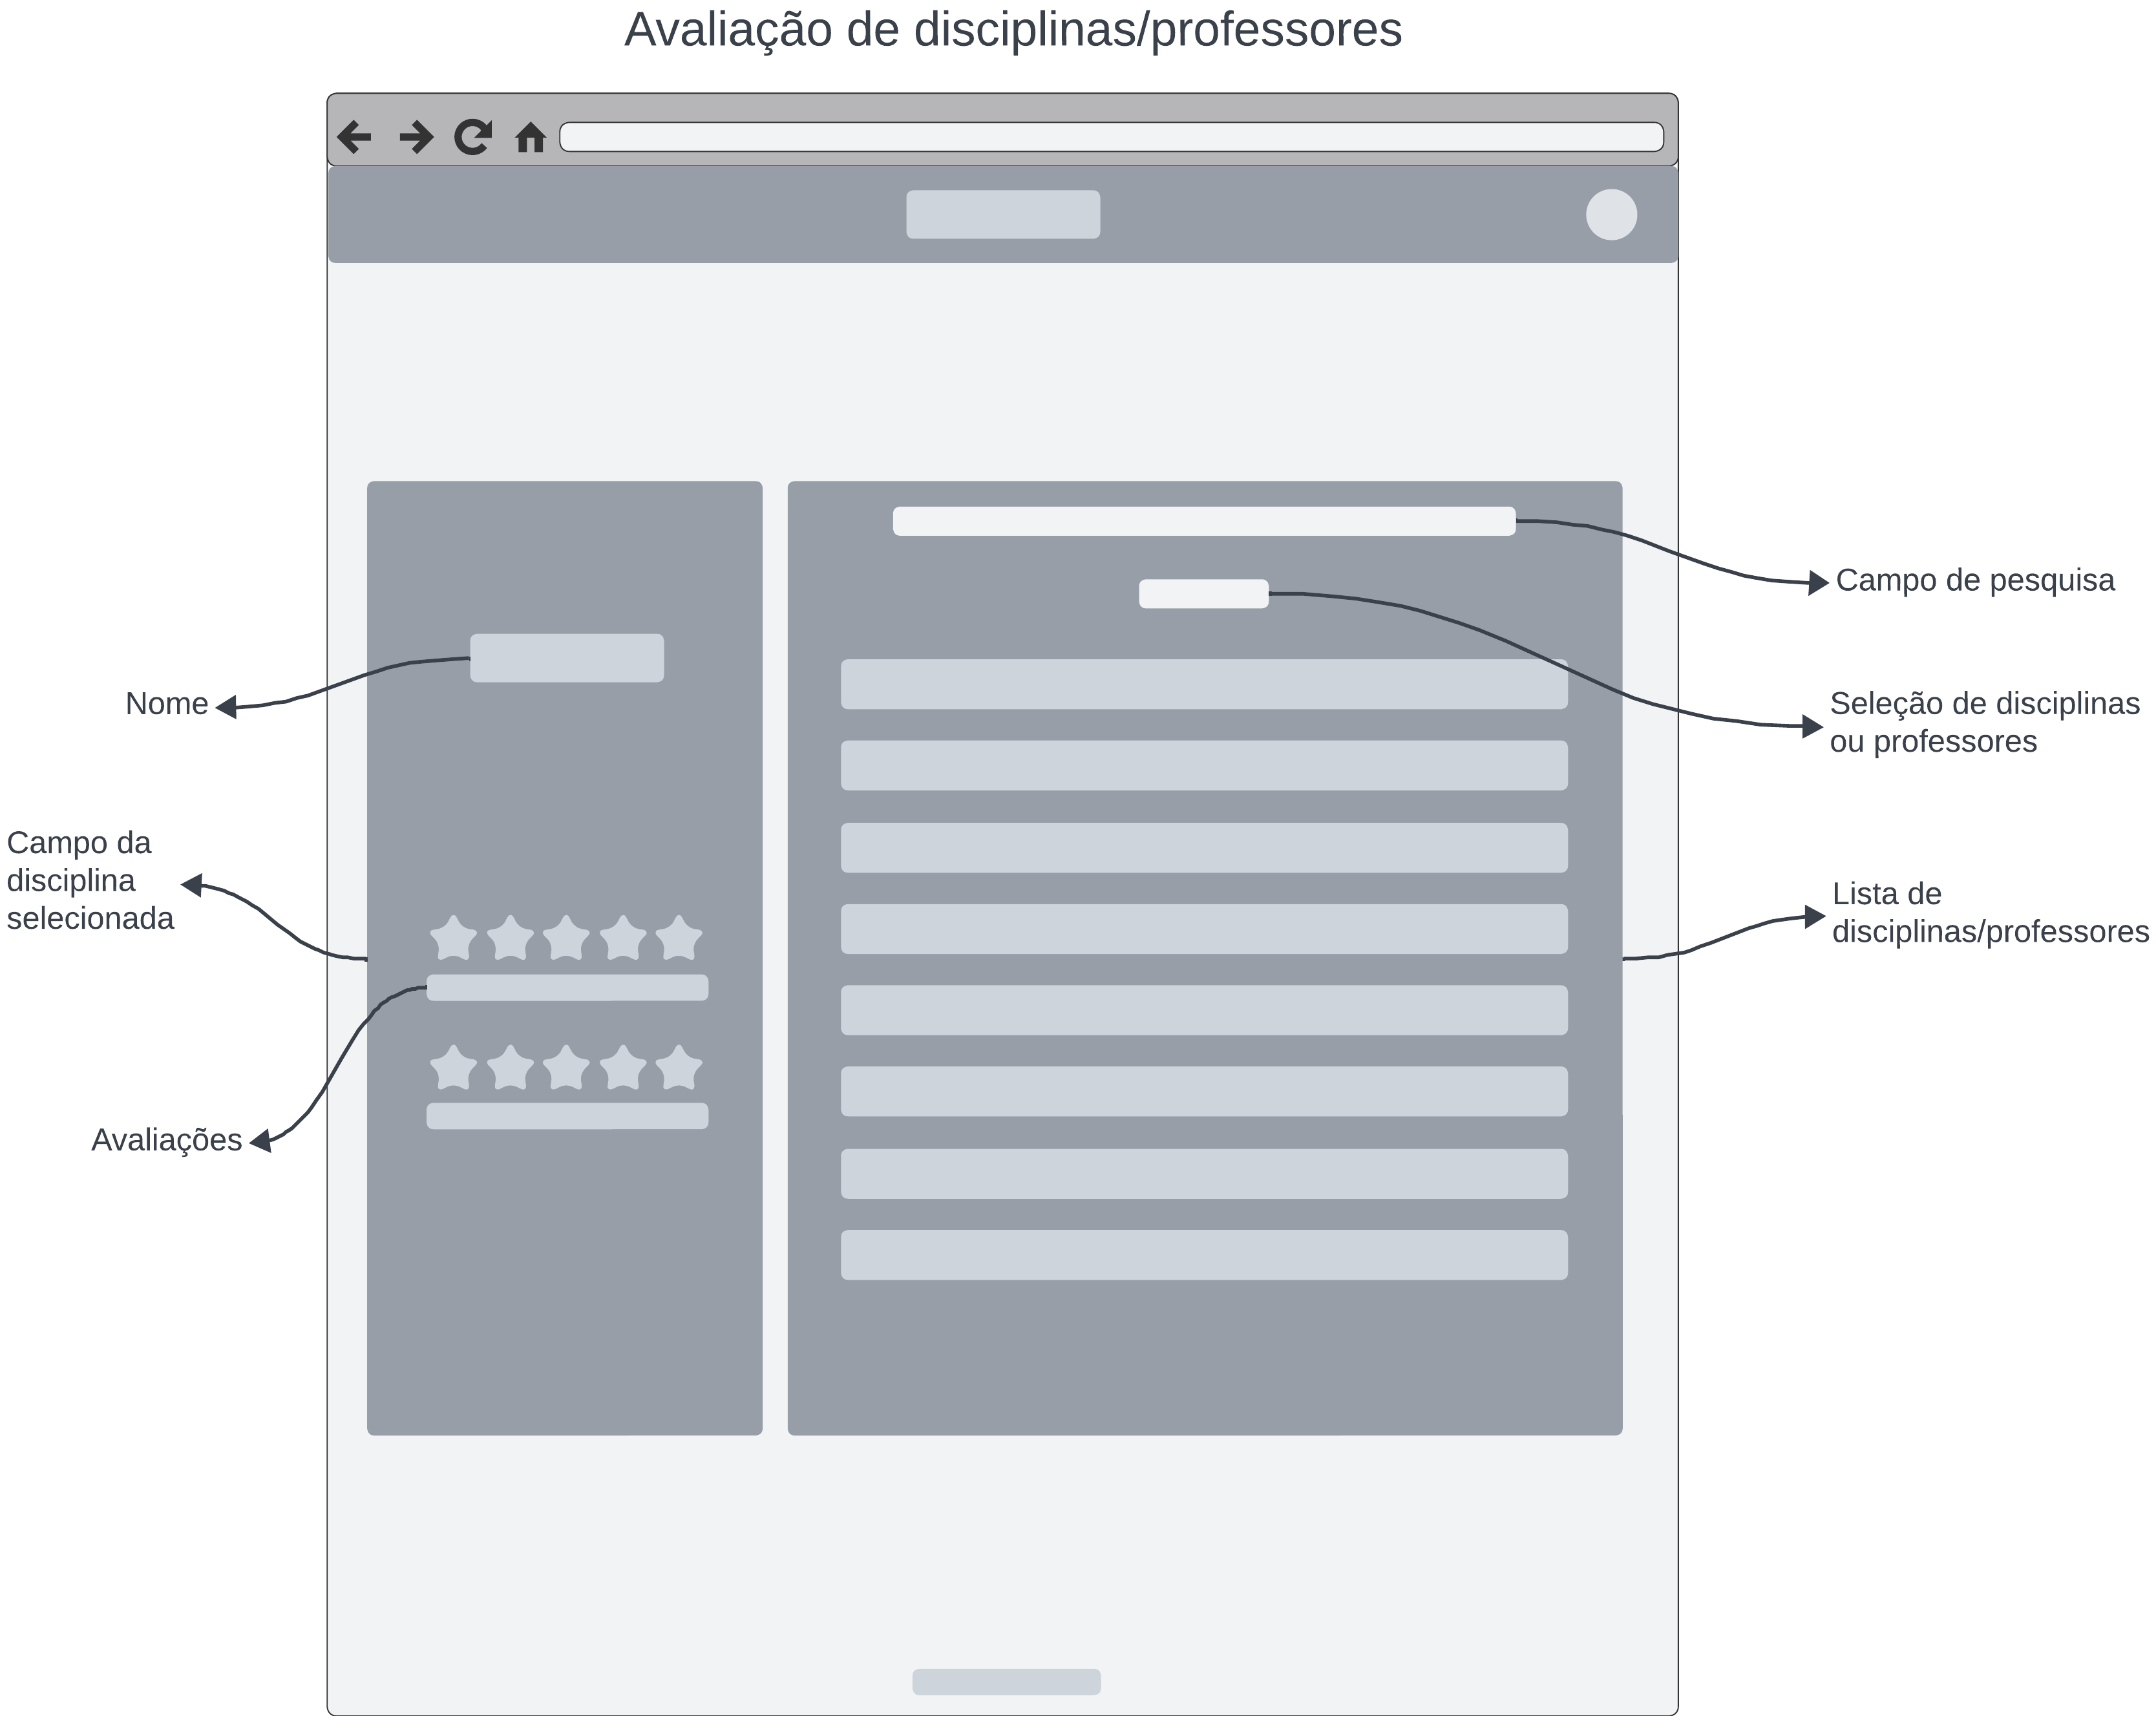
\includegraphics[width=390pt]{figuras/pagina-avaliacao.png}
    \caption{Wireframe da página de avaliação de disciplinas}
    \label{fig:wireframe-pagina-avaliacao}
    \end{center}
\end{figure}
  \chapter{Dados do sistema}
\label{cha:Dados do sistema}

Para satisfazer os requisitos e os casos de uso, foi necessário modelar os dados disponíveis ao sistema e ao algoritmo.

\section{Modelo Entidade-Relacionamento}

A imagem \ref{fig:diagrama-classes} exibe o diagrama do modelo entidade-relacionamento (ER), que descreve os dados no modelos de entidades (coisas de interesse) e seus relacionamentos. O modelo ER segue a notação do Peter Chen \cite{peter-chen}. 

\begin{figure}[ht]
    \begin{center}
    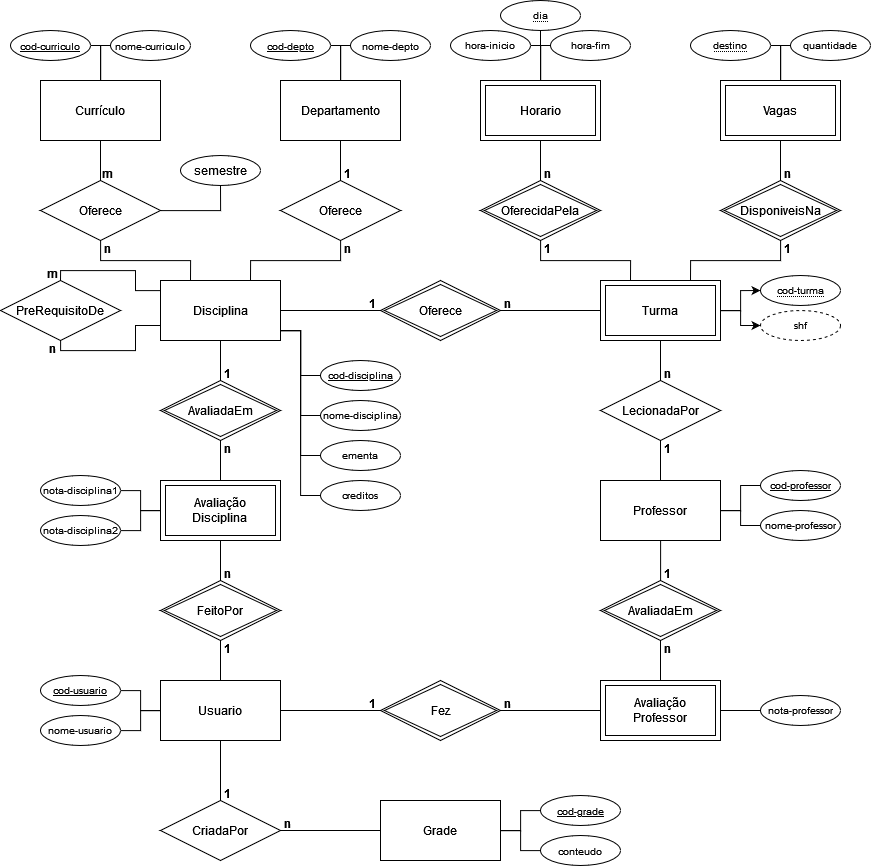
\includegraphics[width=390pt]{figuras/diagrama-er-chen-pdf.png}
    \caption{Diagrama de classes}
    \label{fig:diagrama-classes}
    \end{center}
\end{figure}

\section{Modelo Físico}

A imagem \ref{fig:modelo-fisico} exibe o diagrama físico dos dados com base no modelo ER. Ele representa a estrutura implementada no banco de dados, com suas tabelas e chaves primárias (PK) e chaves estrangeiras (FK).

\begin{figure}[ht]
    \begin{center}
    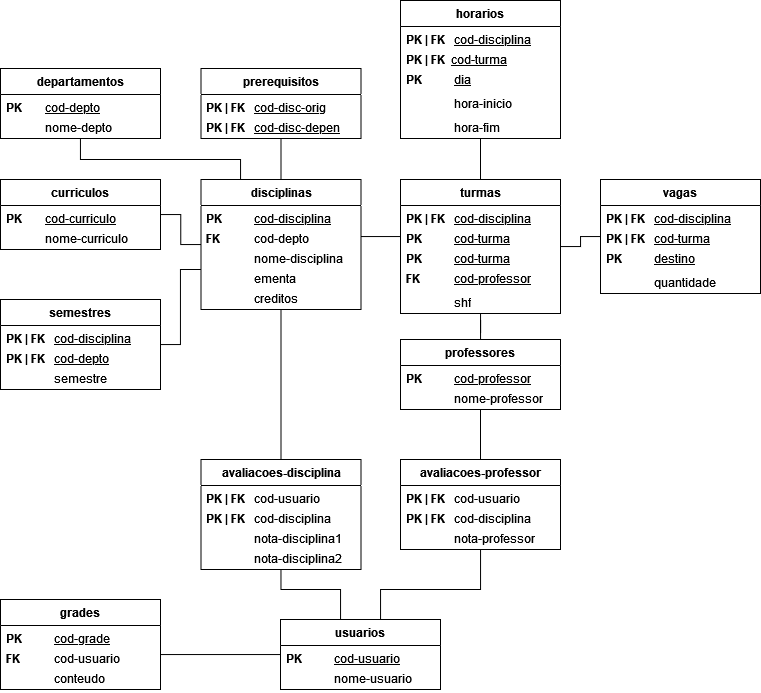
\includegraphics[width=390pt]{figuras/modelo-fisico.png}
    \caption{Modelo físico dos dados}
    \label{fig:modelo-fisico}
    \end{center}
\end{figure}

\section{Dicionario de dados}

aaaaaa a preencher

  \chapter{Construção}
\label{cha:Construção}

\section{Tecnologias utilizadas}
\label{sec:Tecnologias utilizadas}

Para o armazenamento e consulta dos dados, foi utilizado o banco de dados relacional PostgreSQL \cite{site-postgresql}. O PostgreSQL foi escolhido por ser robusto e eficiente, mas fácil e rápido de configurar. 

O sistema foi separado em interface e API (\textit{Application programming interface}, ou interface de programação da aplicação). A coleta dos dados provenientes do Microhorario, a autenticação com o sistema acadêmico universitário e carga/processamento dos históricos foi desenvolvida em serviços menores uma única funcionalidade respecitvamente (microserviços). 

A figura \ref{fig:diagrama-arquitetura} exibe um diagrama da arquitetura do sistema.

\begin{figure}[ht]
    \begin{center}
    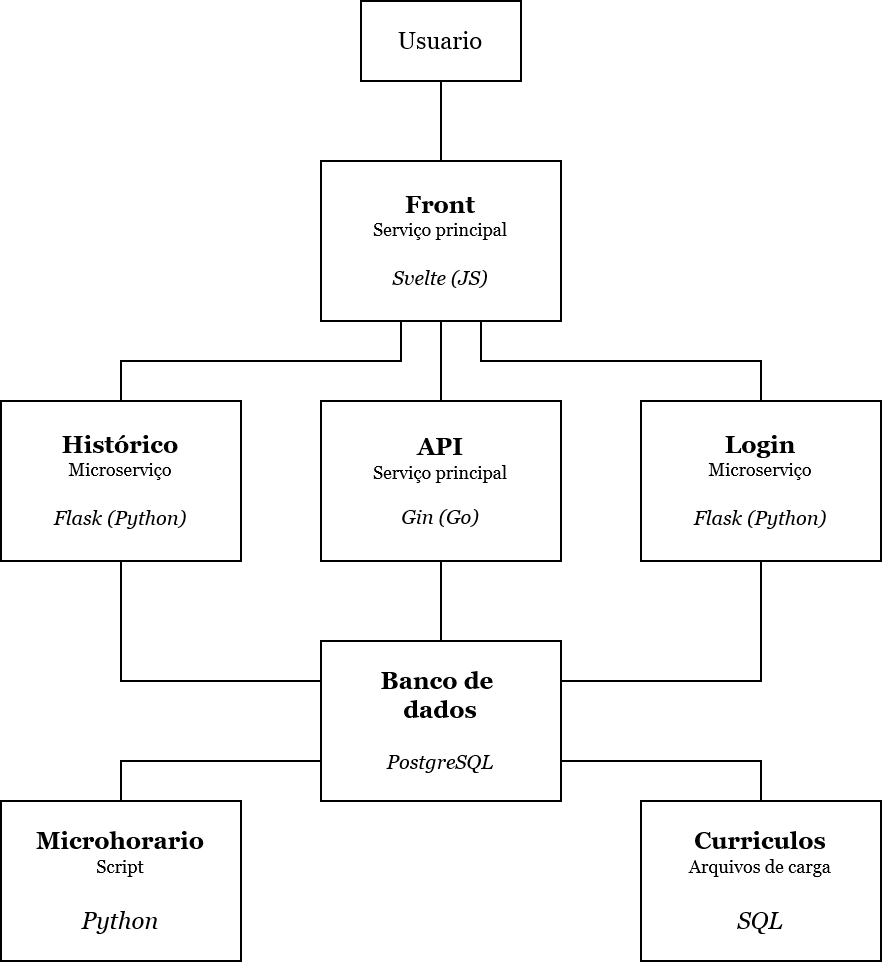
\includegraphics[width=300pt]{figuras/diagrama-arquitetura.png}
    \caption{Diagrama da arquitetura do sistema}
    \label{fig:diagrama-arquitetura}
    \end{center}
\end{figure}

\section{Coleta de dados}
\label{sec:Coleta de dados}

O o modelo lógico representado na figura \ref{fig:modelo-logico} define a construção de catorze tabelas no banco de dados. O trecho de código \ref{cod:sql-create} contém o modelo físico do banco de dados, ou seja o código SQL que define a modelagem das tabelas.

\lstinputlisting[label=cod:sql-create,title={create.sql},caption={Modelo físico},language=SQL]{codigo/10-create.sql}

Observando o modelo físico, é possível observar que é possível observar que as avaliações, históricos e currículos devem ser sempre associados às disciplinas, através das chaves estrangeiras. Portanto, as disciplinas não podem ser excluídas, mesmo que elas não possam não estar sendo oferecidas no semestre atual. Para diferenciar uma disciplina que está sendo oferecida de uma disciplina que não está disponível, basta verificar se ela existe na tabela \verb|turmas|, que é constantemente atualizada conforme as disponibilidades.

No modelo físico, existe a criação de uma tabela \verb|modificacao|, que não estava prevista no modelo lógico. Essa tabela não contém dados relacionais, mas apenas três valores armazenados em uma só linha da tabela. Esses valores representam as datas de coleta das informações das disciplinas e turmas, e se os dados estão em modo de \verb|fallback|, que será explicado depois.

Além dos dados gerados pela interação do usuário, o sistema precisa de dados provenientes da faculdade, como as disciplinas, turmas, professores e currículos. Esses dados são coletados ocasionalmente, exceto os currículos, que foram manualmente costruídos a partir de informações disponíveis nas plataformas da universidade. Como o algoritmo e o sistema foi planejado para alunos do departamento de informática, a quantidade de currículos a ser inserida é pequena. No total, foram inseridos seis currículos: três de engenharia de computação (Currículos 2023, 2018.0 e 2018.1) e três de ciência de computação, disponíveis nas respectivas páginas
\footnote{\url{https://www.puc-rio.br/ensinopesq/ccg/eng_computacao.html}}
\footnote{\url{https://www.puc-rio.br/ensinopesq/ccg/ciencia_computacao.html}}
dos cursos.

Os dados do currículo foram transformados manualmente em um arquivo no formato SQL que insere o código do currículo e constrói uma \verb|PROCEDURE|, um procedimento responsável por inserir as disciplinas referentes ao currículo. As disciplinas estão dentro de uma verb|procedure| pois esta deve ser executada toda vez que uma disciplina nova possa ter sido inserida no banco. Isso é necessário pois a \verb|procedure| armazena somente o código de disciplinas que existem no banco, devido a restrição de chave estrangeira da tabela. Portanto, cada vez que uma disciplina nova é inserida, essa operação precisa ser refeita. O trecho de código \ref{cod:sql-curriculo} contém um exemplo de um dos seis arquivos criados, um para cada currículo.

\lstinputlisting[label=cod:sql-curriculo,title={curriculo-cie-18-0.sql},caption={Exemplo do arquivo de carga de currículos},language=SQL]{codigo/10-curriculos.sql}

Os dados provenientes das disciplinas e turmas são coletados diretamente através do microhorário. Foi criada uma biblioteca Python que permite baixar todos as informações disponíveis no microhorário, e opcionalmente coletar as ementas e pré-requisitos que estão disponíveis em página. A biblioteca baixa os dados das disciplinas e turmas em menos de três segundos, mas pode executar por até 30 minutos para baixar as ementas e pré-requisitos que estão em outro serviço da universidade. Portanto, foi criado um módulo, chamado \verb|microhorario|, que permite atualizar o banco com as informações básicas das disciplinas e turmas, mas que pode ser alterado para atualizar também as ementas e pré-requisitos. Esse módulo foi configurado de forma a ser executado na sua forma mais simples (somente atualiza os dados referentes às turmas) uma vez a cada hora, e executado na forma completa (coleta inclusive as ementas e pré-requisitos) uma vez por dia.

No final de cada período, devido a preparação das disciplinas e turmas para o próximo semestre, o microhorário não disponibiliza dados como quantidade de vagas e quantidade de créditos. Por isso, foi necessário que o sistema e o algoritmo acomodasse essas necessidades temporárias. Nesse caso, a variável de \verb|fallback|, presente na tabela de \verb|modificacao| estará no seu valor verdadeiro. Se o microhorário estiver disponível, essa variável está com seu valor falso.

\subsection{Disciplinas optativas}
Os currículos contém grupos de disciplinas optativas. Cada grupo de disciplinas optativas possuem várias disciplinas, e o aluno deve cursar pelo menos uma delas para que seja considerado o grupo como cursado. Por exemplo, o currículo de 19.0 de Engenharia de Computação determina o grupo de optativa \verb|INF0303|, com as disciplinas \verb|ENG1456 - INTELIGENCIA COMPUT APLICADA| e \verb|INF1771 - INTELIGENCIA ARTIFICIAL|, e o aluno deve necessariamente cursar uma das duas. Essa categoria de disciplinas não foi percebida durante todo o processo de entrevistas, levantamento de requisitos e modelagem do banco. E para implementar essa categoria de forma eficaz, seria necessária uma reestruturação das tabelas do banco de dados, e diversas alterações complexas nos módulos de coleta de dados do microhorário e dos outros serviços, inclusive alterações na biblioteca de consulta ao microhorário citada acima. Portanto, optou-se por não implementar as disciplinas optativas. Em vez disso, as disciplinas relacionadas ao grupo de optativas não são atreladas ao currículo, sendo consideradas eletivas.

\subsection{Co-requisitos}
Durante o desenvolvimento de coleta de dados da ementa, foi observado que algumas disciplinas possuem co-requisitos. Co-requisitos são disciplinas que precisam ser cursadas no mesmo período, conforme a imagem \ref{fig:corequisito}. Como esse atributo foi descoberto no momento que o desenvolvimento já estava em andamento, optou-se por não implementar essa funcionalidade. Em vez disso, nenhuma disciplina possui co-requisitos.

\begin{figure}[ht]
    \begin{center}
    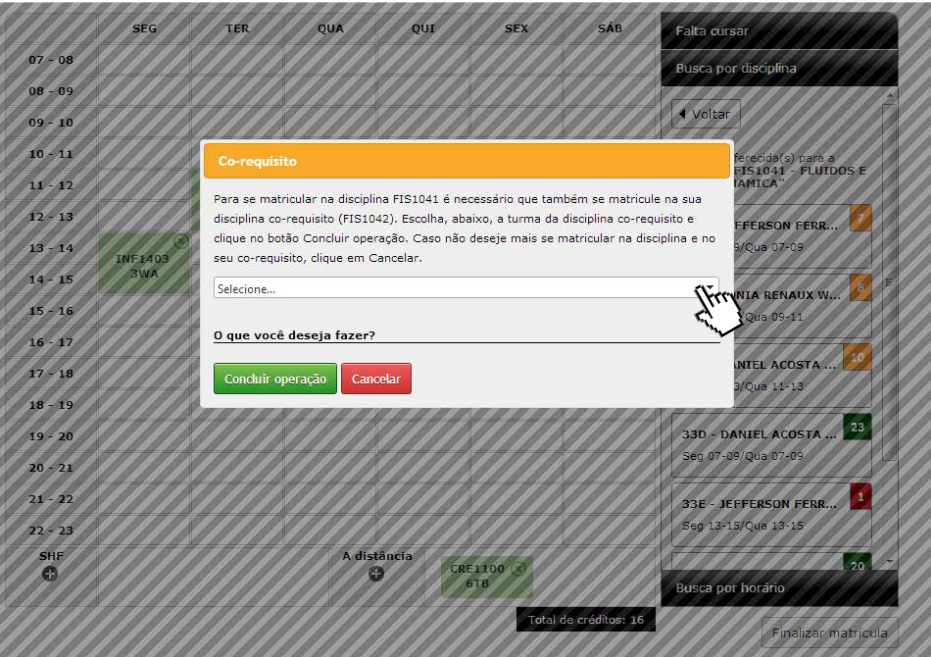
\includegraphics[width=350pt]{figuras/corequisitos.png}
    \caption{Seleção de uma disciplina com co-requisitos durante o processo de matrícula}
    \label{fig:corequisito}
    \end{center}
\end{figure}



\section{Definição e implementação do algoritmo}
\label{sec:Definição e implementação do algoritmo}

O algoritmo busca satisfazer as necessidades apresentadas na tabela \ref{tab:entrevista-criterios-peso}. As entrevistas indicaram a importância de cinco categorias (Conteúdo, Professor, Avaliação, Horário e Opinião). Por isso, o algoritmo foi dividido nessas cinco categorias.

O algoritmo se baseia num valor $V[d,u]$ atribuído a cada disciplina, que indica a relevância da disciplina $d$ para o usuário $u$. O valor $V[d,u] \in [0, 1]$,
sendo 1 o maior grau de relevância da disciplina, e 0 o menor. O cálculo de $V$ é uma média ponderada, conforme a equação \ref{equ:algoritmo-valor}.

\begin{multline}
\label{equ:algoritmo-valor}
    V[d,u] = \\
        P_cV_c[d,u] + P_pV_p[d] + P_oV_o[d] + P_hV_h[d,u] + P_aV_a[d]
\end{multline}

Em que $d$ é uma disciplina, $u$ é um usuário, $P_x$ é o valor de uma das cinco categorias para a disciplina $d$ e o usuário $u$, e $P_x$ é o peso de uma das cinco categorias.

%% valor V_c

O valor $V_c[d,u]$ indica o quão relevante é a disciplina para o usuário de acordo com o seu conteúdo. Para isso, o valor é calculado de acordo com o histórico de outros alunos e com o currículo do aluno, conforme a equação \ref{equ:algoritmo-conteudo}.

\begin{equation}
    V_c[d,u] = 
    \begin{dcases}
        \hfil 1.0 & \text{caso} \: d \in Historico[u] \\ 
        \frac{|\, A_{cursou}[d,u] \,|}{|\,  A_{curriculo}[u] \,|}   & \text{caso} \: A_{curriculo}[u] > 0 \\
        0 & \text{caso contrário}
    \end{dcases} \\[20pt]
    \label{equ:algoritmo-conteudo}
\end{equation}

Em que:

\begin{align*}
    & A_{curriculo}[u] = \forall a \in Alunos \,|\, Curriculo[a] = Curriculo[u] \\
    & A_{cursou}[d,u] = \forall a \in A_{curriculo}[u] \,|\, d \in Cursadas[a] \\
\end{align*}

Em que $d$ é uma disciplina, $u$ é um usuário, $Alunos$ é o conjunto de todos os usuários cadastrados no sistema, $Curriculo[u]$ é o currículo do usuário $u$, e $Cursadas[u]$ é o conjunto de disciplinas que o aluno $u$ cursou. Em resumo, o valor $V_c[d,u]$ é o valor máximo caso a disciplina deve ser cursada pelo usuário, ou sendo uma eletiva é a proporção de alunos do mesmo currículo que fizeram esta disciplina. Essa proporção indica se o conteúdo é relevante para alunos semelhantes ao usuário.

%% Valor V_p

O valor $V_p[d]$ indica o quão relevante é a disciplina para o usuário de acordo com o professor. Para isso, o valor é calculado de acordo com as avaliações dos professores das turmas das disciplinas, conforme a equação \ref{equ:algoritmo-professor}.

\begin{equation}
    V_p[d] = \frac{\sum_{p \in P[d]} \displaystyle  \frac{\sum_{a \in Avs[p]} a}{| Avs[p] |}}{| P[d] |} \,/\, 5
    \label{equ:algoritmo-professor}
\end{equation}

Em que $d$ é uma disciplina, $P[d]$ é o conjunto dos professores que lecionam a disciplina $d$, e $Avs[p]$ representa o conjunto das avaliações dos usuários do professor $p$. Em resumo, o valor $V_p[d,u]$ é a média das avaliações de todos os professores que estão lecionando a disciplina, com o valor entre $0$ e $1$.

%% Valor V_o

O valor $V_o[d]$ indica o quão relevante é a disciplina para o usuário de acordo com a opinião dos alunos. A equação é semelhante ao cálculo apresentado na equação \ref{equ:algoritmo-professor}. Porém, nesse caso, é levado em conta a média das avaliações das próprias disciplinas, conforme a equação \ref{equ:algoritmo-opiniao}.

\begin{equation}
    V_p[d] = \frac{\sum_{a \in Op[d]} a} {| Op[d] |} \,/\, 5
    \label{equ:algoritmo-opiniao}
\end{equation}

Em que $d$ é uma disciplina, e $Op[d]$ é o conjunto das avaliações dos usuários da disciplina $d$.

%% Valor V_h

O valor $V_h[d,u]$ indica o quão relevante é a disciplina para o aluno de acordo com o horário. Para isso, o valor é calculado de acordo com os horários ocupados na grade do usuário e os horários das disciplinas, conforme a equação \ref{equ:algoritmo-horario}

\begin{equation}
    V_h[d,u] = 
    \begin{dcases}
        \frac{|\, T_{possiveis}[d,u] \,|}{|\,  T[d] \,|}   & \text{caso} \: T[d] > 0 \\
        \hfil 0 & \text{caso contrário}
    \end{dcases} \\[20pt]
    \label{equ:algoritmo-horario}
\end{equation}

Em que $d$ é uma disciplina, $u$ é um usuário, $T_{possiveis}[d,u]$ é o conjunto de turmas da disciplina $d$ que se encaixam na grade do usuário $u$, e $T[d]$ é a quantidade de turmas da disciplina $d$. Em resumo, $V_h[d, u]$ é a porcentagem de turmas da disciplina que se encaixam na grade do usuário.

Por último, o valor $V_a[d]$ indica o quão relevante é a disciplina para o aluno de acordo com os graus (a nota final, considerando as provas do aluno durante o semestre) da disciplina. O cálculo é semelhante às equações \ref{equ:algoritmo-professor} e \ref{equ:algoritmo-opiniao}, conforme a equação \ref{equ:algoritmo-avaliacao}.

\begin{equation}
    V_p[d] = \frac{\sum_{g \in Graus[d]} g} {| Graus[d] |} \,/\, 100 
    \label{equ:algoritmo-avaliacao}
\end{equation}

Em que $d$ é uma disciplina e $Graus[d]$ é o conjunto das notas da disciplina $d$.

Para obter todos os valores dos conjuntos citados nas equações anteriores, foi criada uma consulta SQL que obtém todos os valores de uma só vez. O trecho de código \ref{cod:sql-algoritmo} contém a consulta por completo. Antes de executar, são substituidos os valores \verb|@usuario| pelo código do usuário, e o valor \verb|@escolhas| por um trecho de código SQL referente às escolhas de turmas de disciplinas na grade atual do aluno.

\lstinputlisting[label=cod:sql-algoritmo,title={algoritmo.sql},caption={Consulta dos dados para o algoritmo},language=SQL]{codigo/10-algoritmo.sql}

Por fim, os pesos $P_x$ da média ponderada foram baseados na tabela \ref{tab:entrevista-criterios-peso}. Cada peso é a soma dos pesos dos critérios, de acordo com as equações a seguir.

\begin{align}
    & P_c = \frac{41}{41 + 19 + 8 + 28 + 21} \\[10pt]
    & P_p = \frac{28}{41 + 19 + 8 + 28 + 21} \\[10pt]
    & P_o = \frac{ 8}{41 + 19 + 8 + 28 + 21} \\[10pt]
    & P_h = \frac{19}{41 + 19 + 8 + 28 + 21} \\[10pt]
    & P_a = \frac{21}{41 + 19 + 8 + 28 + 21}
\end{align}

\section{Implementação da API}
\label{sec:Implementação da API}

A API é responsável por servir disponibilizar à interface os dados de forma organizada e eficaz. Foi estudada a implementação da API em quatro possíveis frameworks em três diferentes linguagens:
\textit{Django} \cite{site-django}, \textit{Flask} \cite{site-flask}, \textit{Gin} \cite{site-gin} e \textit{Rocket} \cite{site-rocket}. Cada um dos frameworks possui suas vantagens e desvantagens.

O framework \textit{Django} é um \textit{Web Framework} completo, que possui múltiplas funcionalidades pré-configuradas, possui uma interface de comunicação com banco de dados bem robusta. O framework \textit{Flask} por sua vez não possui muitas funcionalidades imbutidas, e depende da instalação de pacotes externos para ampliar suas funcionalidades. Ambos os frameworks são desenvolvidos na linguagem Python, o que torna o desenvolvimento mais fácil, mas reduz performance do funcionamento, por ser uma linguagem interpretada.

O framework \textit{Rocket} é desenvolvido na linguagem Rust \cite{site-rust}, conhecida por ser rápida e segura, por possuir um abordagem de manipulação de memória diferente de outras linguagens. Porém, Rust possui uma alta curva de aprendizado, dificultando o desenvolvimento do código.

Por fim, o framework \textit{Gin} é desenvolvido na linguagem Go \cite{site-go}, conhecida por bem eficiente, útil para o desenvolvimento de APIs pelo sua capacidade de multiprocessamento, e fácil de usar. Por isso, esse framework foi escolhido para a API do sistema.

A API disponibiliza a documentação completa de todas as suas rotas, com as respectivas entradas e saídas, conforme a figura \ref{fig:api}.

\begin{figure}[ht]
    \begin{center}
    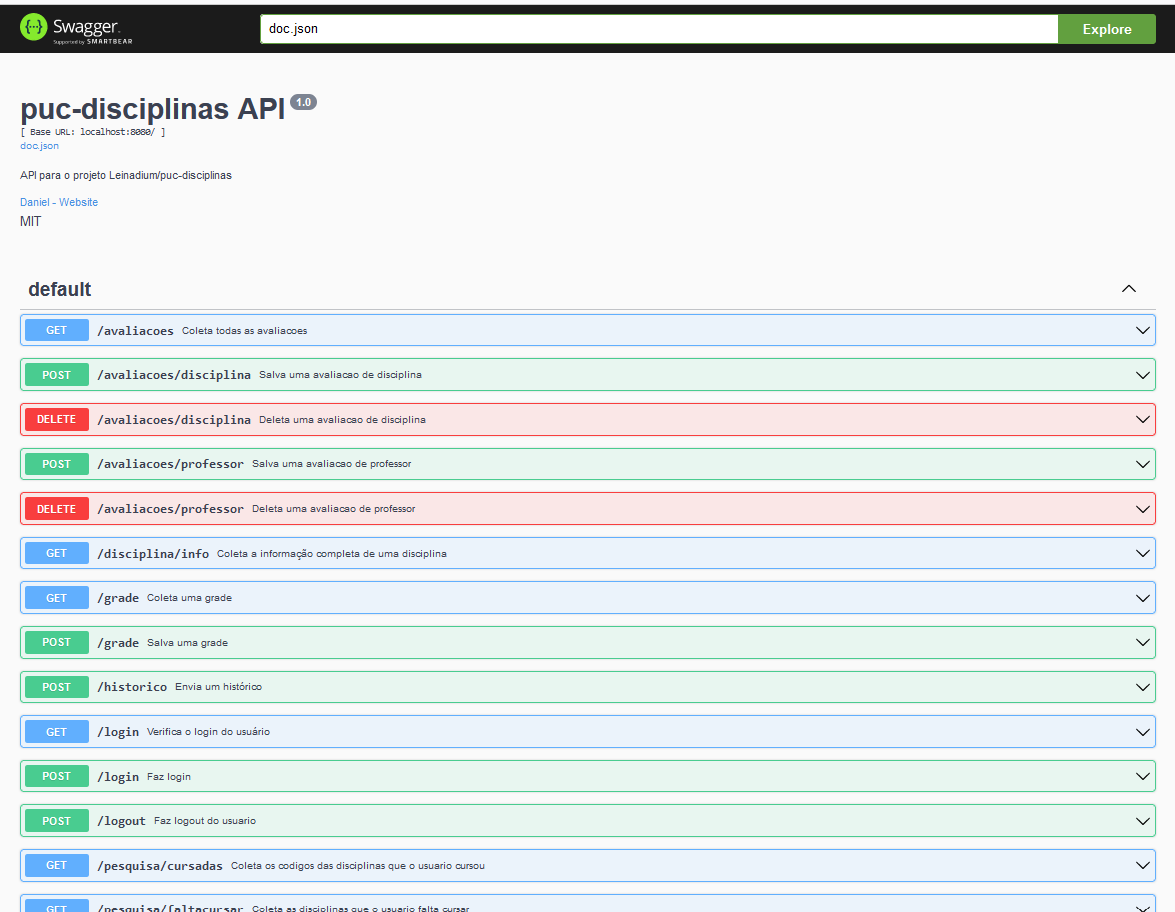
\includegraphics[width=360pt]{figuras/api.png}
    \caption{Documentação da API}
    \label{fig:api}
    \end{center}
\end{figure}

\section{Implementação dos microserviços}
\label{sec:Implementação dos microserviços}

Os serviços de autenticação, e de carga e processamento dos históricos dos alunos são processos separados da API. Ambos foram desenvolvidos na linguagem Python, por sua facilidade de processamento dos dados, e por não haver a necessidade uma performance ótima. Esses utilizam o framework Flask para disponibilizar os serviços, por serem serviços bem simples.

O serviço de autenticação se comunica com o sistema acadêmico universitário (SAU). Existe uma API para autenticação dos alunos da universidade, mas é restrita para os serviços interno da mesma. Por isso, o serviço de autenticação implementado simula um aluno autenticando-se no portal \footnote{Disponível em: \url{https://www.puc-rio.br/ensinopesq/academicas/}, Sistemas Acadêmicos - SAU} do SAU, e verifica se a autenticação foi efetuada com sucesso.

O serviço de carga dos históricos precisa receber como entrada a página do histórico do usuário. É possível coletar o histórico de forma automática, acessando o portal do SAU também simulando um usuário. Porém, como essa interação com o SAU não seria transparente com o usuário, sendo executado de forma oculta, não era a melhor opção. Por isso, optou-se pelo usuário salvando uma cópia da página do seu histórico, e submtendo-o através da interface, que se comunica com o serviço de carga e processamento dos históricos. 

\section{Implementação da interface}
\label{sec:Implementação da interface}

A interface foi implementada utilizando o framework \textit{Svelte}, que permite desenvolver páginas interativas baseadas em componentes. A programação é feita utilizando um misto de Javascript e HTML, que é compilada em pacotes Javascript pequenos que são interpretados pelo navegador de internet. 

Como foi necessário desenvolver pelo menos três páginas diferentes, conforme o wireframe do capítulo \ref{cha:Wireframe}, foi utilizado o framework \textit{SvelteKit} \cite{site-sveltekit}. Este permite disponibilizar páginas desenvolvidas em Svelte em diferentes rotas, além de outras possibilidades, como SSR (\textit{Server-Side Rendering}, ou renderização no servidor), que permite reduzir o esforço do navegador do usuário ao construir inicialmente a página no servidor. 

A seguir estão algumas imagens da interface implementada do sistema. A figura \ref{fig:tela-inicial-impl} mostra a tela inicial, com um menu de seleção para a página de grade e de avaliações. As figuras \ref{fig:tela-grade-impl} e \ref{fig:detalhe-turmas-impl} exibem a interface de criação de grade horária. 
Na figura \ref{fig:tela-grade-impl} é possível observar a mensagem de aviso, caso os dados completos do microhorário estejam indisponíveis.

\begin{figure}[ht]
    \begin{center}
    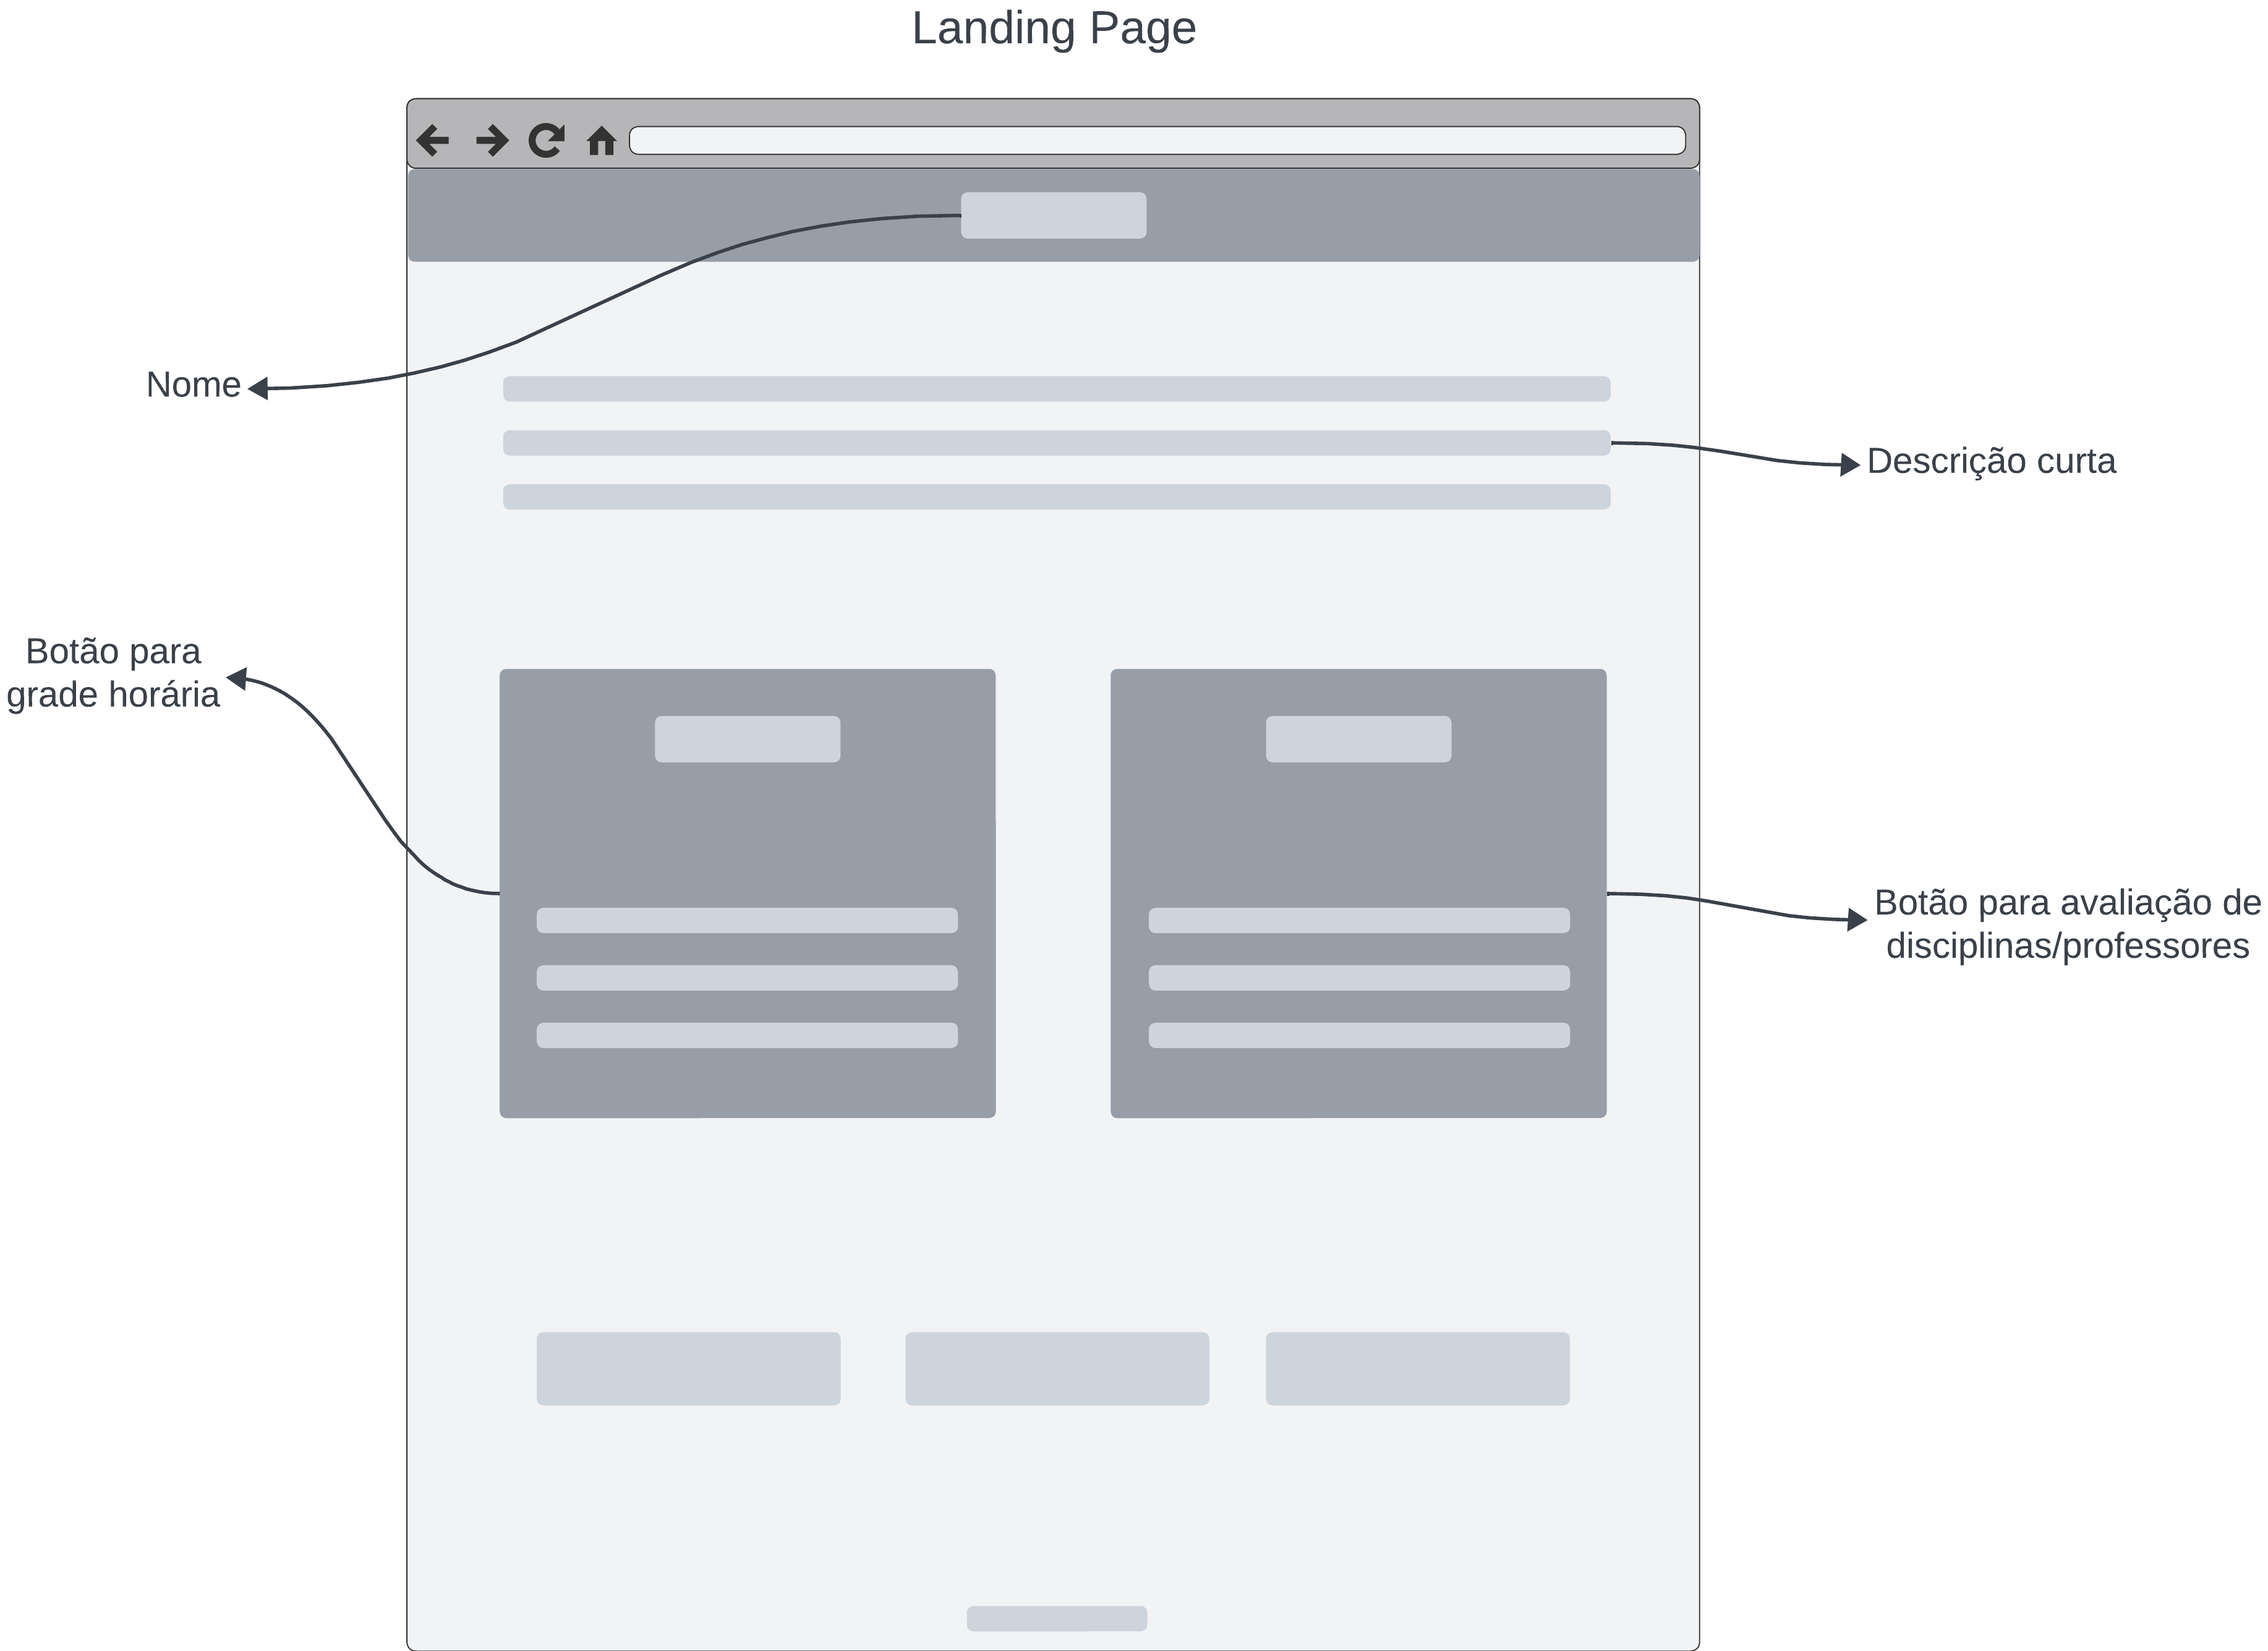
\includegraphics[width=360pt]{figuras/tela-inicial.png}
    \caption{Implementação da tela inicial da interface}
    \label{fig:tela-inicial-impl}
    \end{center}
\end{figure}

\begin{figure}[ht]
    \begin{center}
    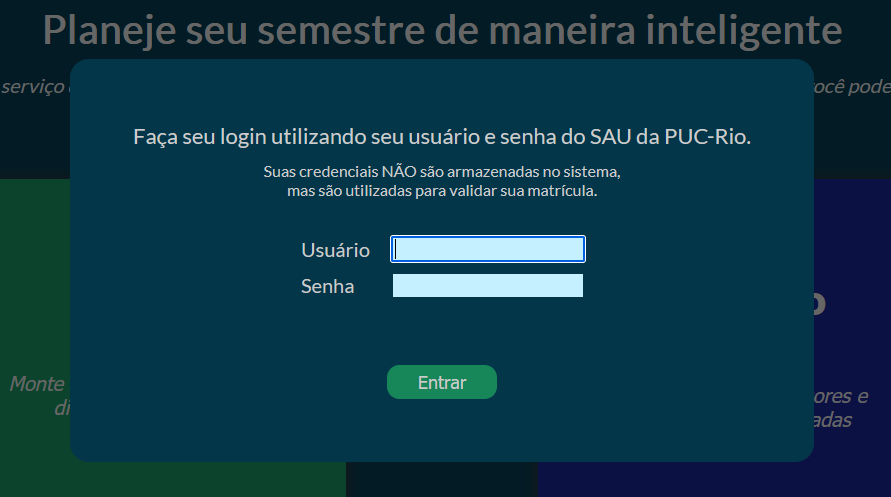
\includegraphics[width=360pt]{figuras/autenticacao-usuario.png}
    \caption{Implementação da tela de autenticação do usuário}
    \label{fig:tela-autenticacao-impl}
    \end{center}
\end{figure}

\begin{figure}[ht]
    \begin{center}
    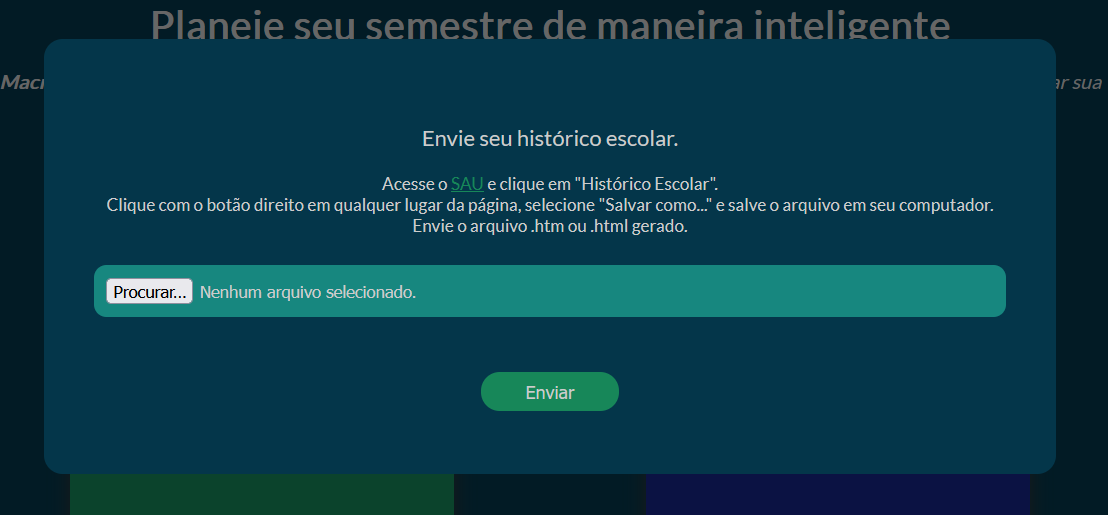
\includegraphics[width=360pt]{figuras/cadastro-historico.png}
    \caption{Implementação da tela de cadastro de histórico}
    \label{fig:tela-historico-impl}
    \end{center}
\end{figure}

\begin{figure}[ht]
    \begin{center}
    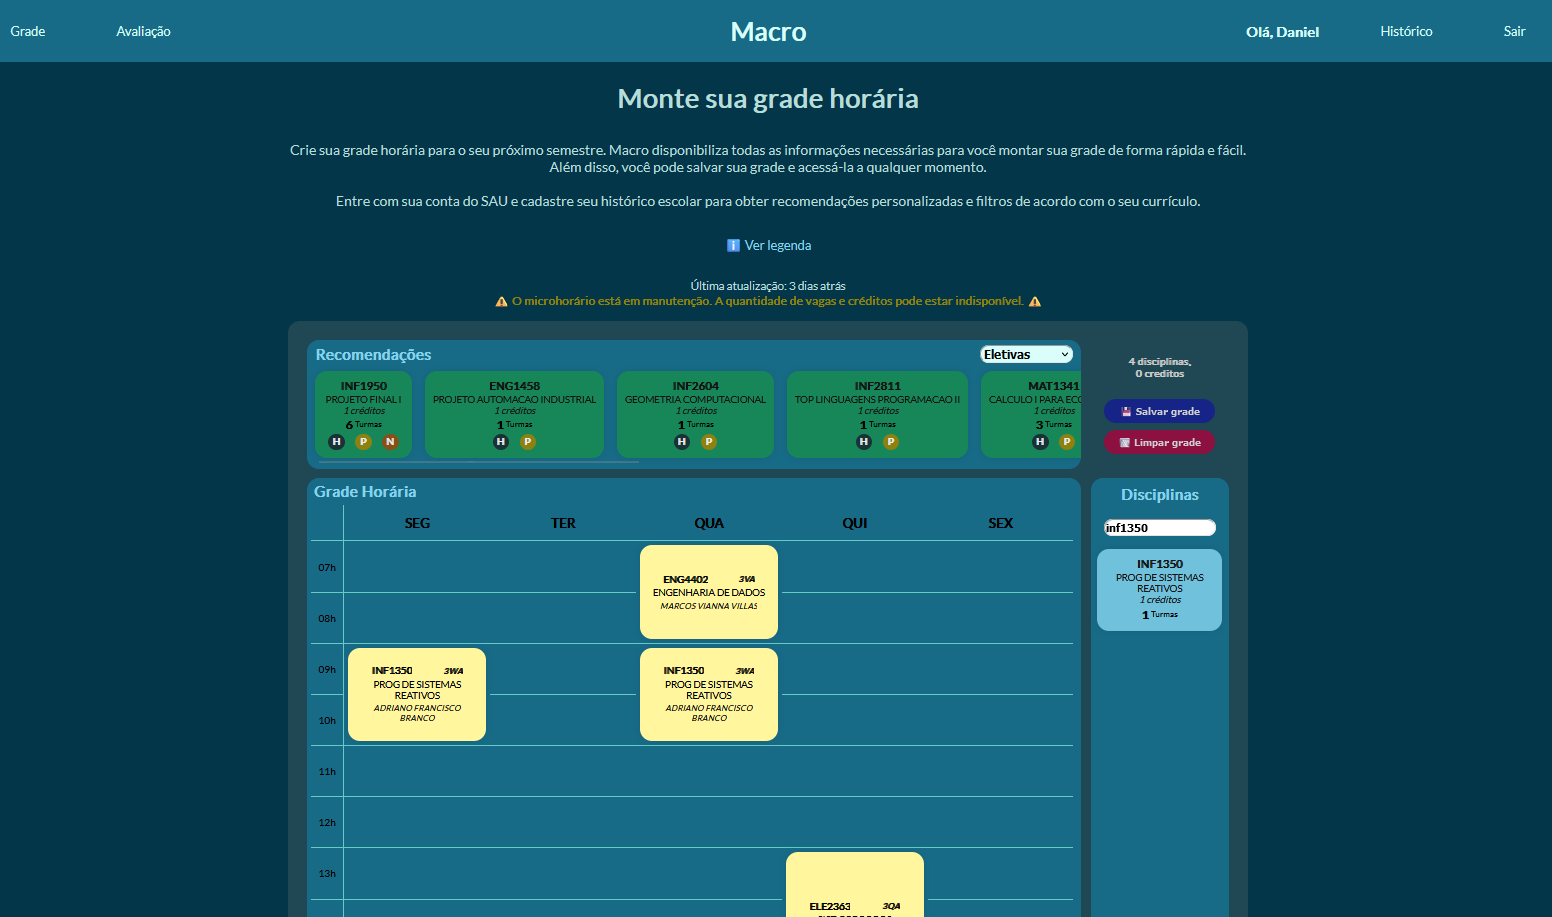
\includegraphics[width=360pt]{figuras/tela-grade.png}
    \caption{Implementação da tela de criação de grade da interface}
    \label{fig:tela-grade-impl}
    \end{center}
\end{figure}

\begin{figure}[ht]
    \begin{center}
    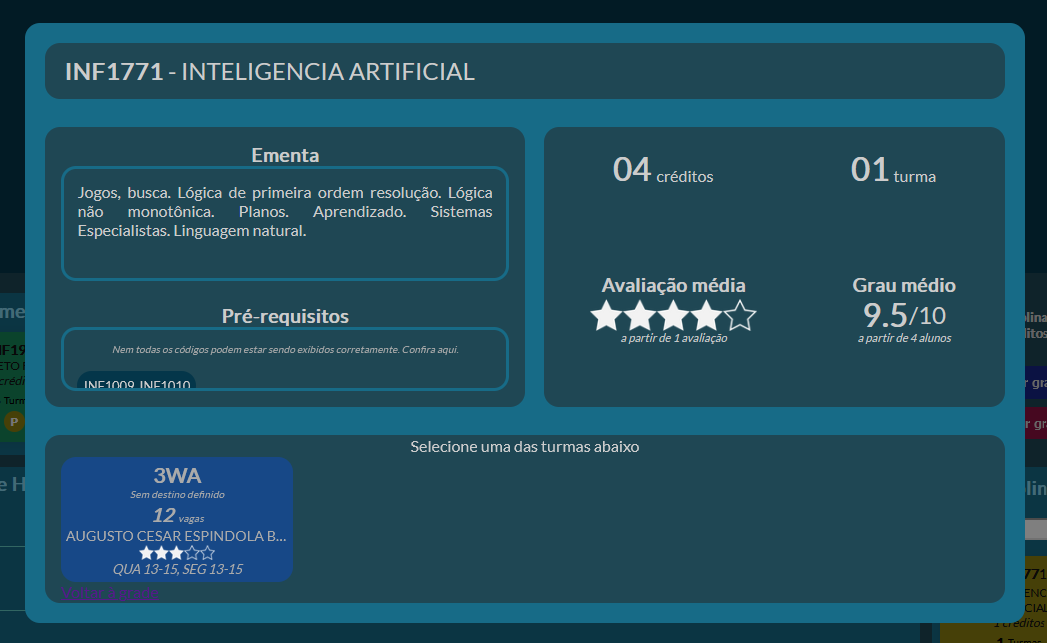
\includegraphics[width=360pt]{figuras/detalhe-turma.png}
    \caption{Detalhes de uma disciplina na interface, exibido ao selecionar uma disciplina}
    \label{fig:detalhe-turmas-impl}
    \end{center}
\end{figure}

\begin{figure}[ht]
    \begin{center}
    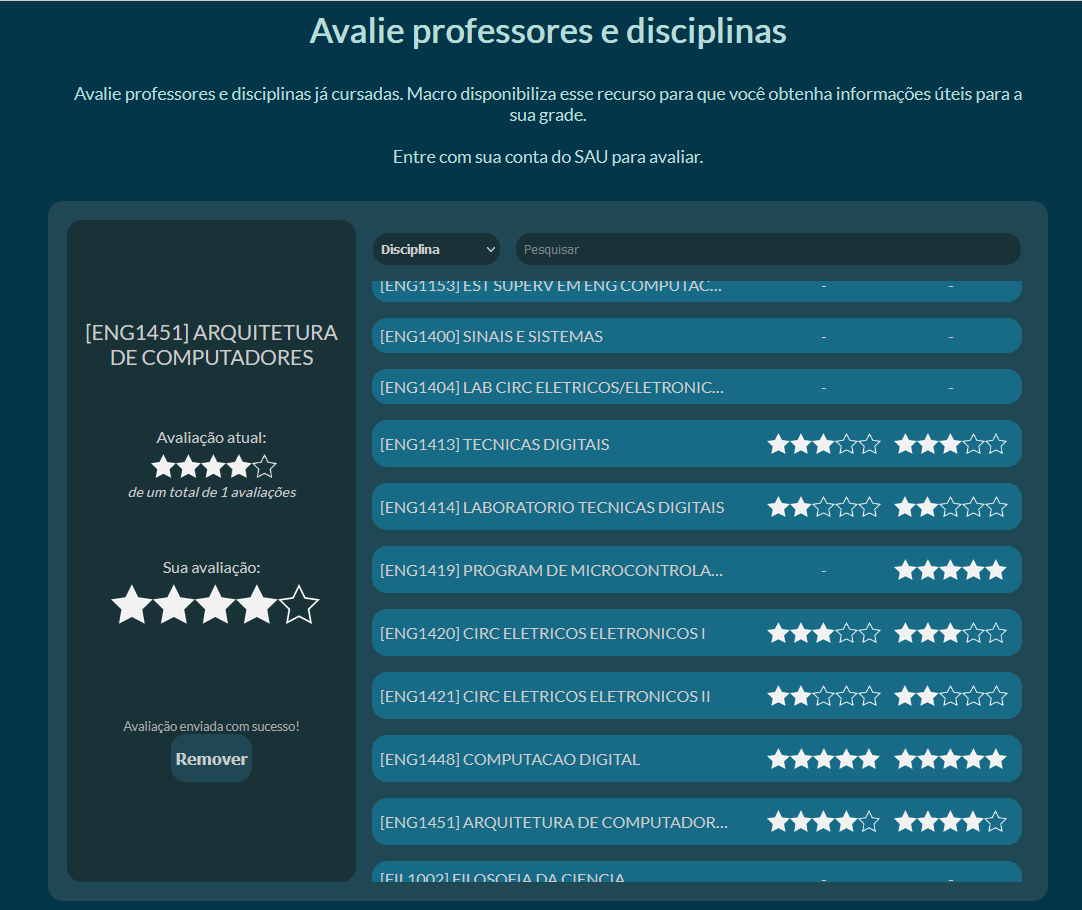
\includegraphics[width=360pt]{figuras/tela-avaliacoes.png}
    \caption{Implementação da tela de avaliação da interface}
    \label{fig:tela-avaliacao-impl}
    \end{center}
\end{figure}

As disciplinas recomendadas podem possuir informações extras. A figura \ref{fig:legenda-interface} mostra uma legenda disponível no sistema explicando as informações exibidas. A figura explica que uma disciplina pode estar sendo recomendada devido a 5 categorias, que estão associadas aos pesos explicados na seção \ref{sec:Definição e implementação do algoritmo}.

\begin{figure}[ht]
    \begin{center}
    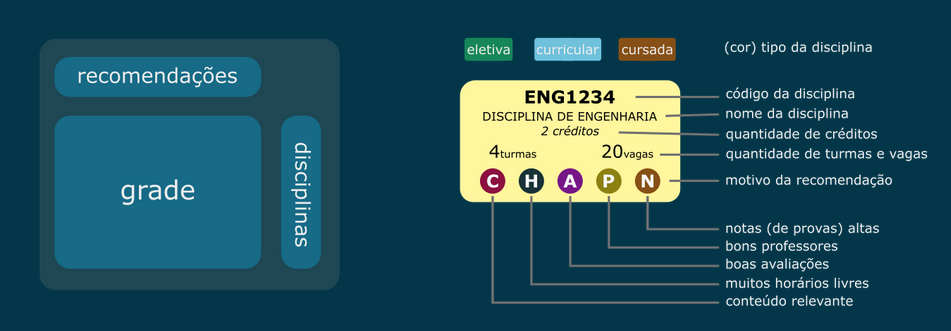
\includegraphics[width=360pt]{figuras/legenda-interface.png}
    \caption{Legenda da interface de criação de grade horária}
    \label{fig:legenda-interface}
    \end{center}
\end{figure}
  \chapter{Testes}
\label{cha:Testes}

Afim de satisfazer todos os requisitos descritos no capítulo \ref{cha:Requisitos}, foram efetuados testes do sistema e algoritmo durante toda a fase de desenvolvimento. Esses testes eram efetuados de maneira não estruturada, apenas para testar todos os possíveis casos de erro. Foi considerada a metodologia de \textit{Desenvolvimento orientado a testes}, que planeja o desenvolvimento primeiro de testes unitários e de integração, para depois o desenvolvimento da aplicação em si. Porém, a implantação dessa metodologia costuma aumentar consideravelmente o tempo de desenvolvimento de aplicações, por isso ela não foi implementada.

Para verificar os requisitos RF01-06, foi testado se o algoritmo recebia todos os parâmetros necessários, e se retornava adequadamente quando os parâmetros não eram satisfeitos. Como a implementação do algoritmo é um modelo matemático, pode-se observar que o requisito RNF2 (que determina que o algoritmo deve retornas os mesmos resultados para as mesmas entradas) foi atendido com sucesso.

Foram efetuados testes de performance, para verificar se os requisitos RNF1 e RNF3 foram satisfeitos. A figura \ref{fig:teste-performance} representa um teste de performance, com 40 usuários simultâneos autenticados solicitando recomendações diferentes a cada 1-5 segundos. É possível observar que o tempo médio de resposta das recomendações foi 20 milisegundos, e não houve nenhuma falha no sistema ou algoritmo. O teste de performance foi desenvolvido usando o framework \textit{Locust} \cite{site-locust}, utilizando a linguagem Python.

\begin{figure}[ht]
    \begin{center}
    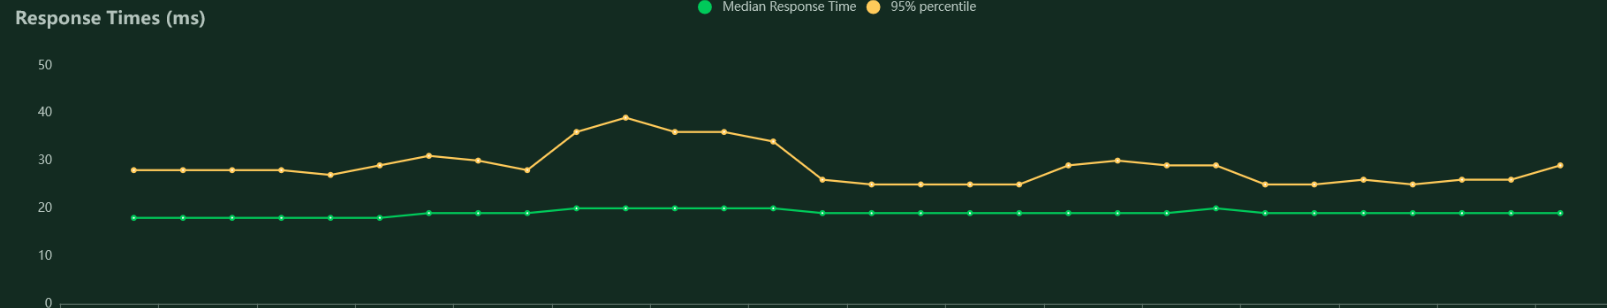
\includegraphics[width=390pt]{figuras/teste-performance.png}
    \caption{Teste de performance da recomendação}
    \label{fig:teste-performance}
    \end{center}
\end{figure}

Ao ter-se uma versão com todas os requisitos atendidos, o processo de testes com os usuários deu-se inicío. A metodologia dos testes foi:

\begin{enumerate}
    \item Apresentar a ideia do sistema e do algoritmo de recomendação;
    \item Apresentar todas as possíveis funcionalidades do sistema;
    \item Criar uma grade horária como exemplo, utilizando-se de todas as funcionalidades do sistema;
    \item Permitir que o usuário faça sua autenticação e crie um grade horária;
    \item Ouvir o feedback do usuário.
\end{enumerate}

O processo de testes com os usuários não foi um simples. Apesar de o sistema possuir todas as suas funcionalidades, o design e as interações ainda estavam incompletas, o que dificultava o entendimento do usuário quanto às funcionalidades. Nem todas as possibilidades estavam bem descritas, e só foram compreendidas por completo após explicações detalhadas.

Os resultados dos testes estão descritos no capítulo \ref{cha:Uso real}.
  \chapter{Uso real}
\label{cha:Uso real}

Ao ter-se uma versão com todas os requisitos atendidos, o processo de testes com os usuários deu-se inicío. A metodologia dos testes foi:

\begin{enumerate}
    \item Apresentar a ideia do sistema e do algoritmo de recomendação;
    \item Apresentar todas as possíveis funcionalidades do sistema;
    \item Criar uma grade horária como exemplo, utilizando-se de todas as funcionalidades do sistema;
    \item Permitir que o usuário faça sua autenticação e crie um grade horária;
    \item Ouvir o feedback do usuário.
\end{enumerate}

Os testes foram realizados durante o processo de desenvolvimento e aprimoramento da interface. Por isso, alguns testes foram prejudicados pela qualidade da interface, que possuia todas as funcionalidades previstas, mas não de forma clara.

Foram entrevistados seis alunos do Departamento de Informática, três de engenharia de computação e três de ciência da computação. Cada aluno estava em um período diferente da sua trajetória, variando do sexto semestre do curso até mais de dez semestres.

Os resultados foram satisfatórios. Todos aprovaram a ideia do algoritmo de recomendação, do sistema de auxílio à criação da grade horária e do sistema de avaliação de disciplinas e professores. A seguir estão algumas sugestões fornecidas pelos usuários após testarem o sistema que não foram modeladas como requisitos. Algumas das ideias foram implementadas posteriormente, enquanto outras serão implementadas em uma etapa futura.

\begin{enumerate}
    \item \textbf{Exibir quantas disciplinas curriculares são trancadas por uma disciplina}: Essa sugestão consiste em exibir a quantidade de disciplinas que uma disciplina bloqueia através dos seus pré-requisitos. Esse número poderia inclusive ser utilizado na fórmula de recomendação afetando $P_c$. Porém ela não foi implementado devido a complexidade do cálculo, que deve ser implementado de maneira recursiva e de preferência, pré-calculado durante o momento de inserção de novas disciplinas.
    
    \item \textbf{Mostrar a quantidade de créditos na grade sendo construída}: Essa sugestão consiste em mostrar a soma dos créditos das disciplinas das turmas selecionadas na grade. Essa sugestão, por sua facilidade de implementação, foi adicionada pouco tempo depois da entrevista. A quantidade de créditos pode ser visualizada acima do botão de salvar grade horária na interface final.
    
    \item \textbf{Exibir quais disciplinas já foram cursadas na lista lateral}: Essa sugestão consiste em diferenciar as disciplinas já cursadas na lista lateral. Essa sugestão foi julgada como importante, e como já havia uma rota na API que disponibiliza quais disciplinas já foram cursadas pelo aluno, esta sugestão foi implementada pouco tempo depois.

    \item \textbf{Filtrar disciplinas por departamento}: Essa sugestão consiste em permitir filtrar as disciplinas na lista lateral pelos seus departamentos. O sistema atual armazena os departamentos das disciplinas, mas não os utiliza em nenhum lugar. Como essa sugestão envolve várias alterações na interface para permitir essa funcionalidade, essa sugestão será imeplementada em um momento futuro.
    
    \item \textbf{Exibir disciplinas não recorrentes}: Nem todas as disciplinas eletivas são oferecidas em todos os períodos. Essa sugestão consiste em exibir dos períodos oferecidos da disciplina, e destacá-la caso ela não tenha sido oferecida no último semestre. Como essa sugestão envolve uma reformulação geral das tabelas do banco de dados, das consultas à API e da interface, optou-se por não implementar essa sugestão nesse momento. 
\end{enumerate}

Foram feitas outras sugestões que envolviam pequenas alterações na interface que não afetavam o funcionamento do sistema ou algoritmo, que foram implementadas ou não de acordo com o nível de complexidade.
  \chapter{Conclusão}
\label{cha:Conclusão}

A partir da construção e dos testes com os usuários, entendeu-se que objetivo do projeto de auxiliar alunos em seus períodos de matrícula foi alcançado.
Ter um sistema para planejar sua matrícula com todas as informações necessárias organizadas em um só lugar, em vez de em três ou quatro serviços diferentes, é inovador
para esta universidade. O algoritmo de recomendação cumpre o seu papel em recomendar disciplinas se utilizando de diversas fontes de informação, facilitando
o planejamento do usuário aluno da universidade.

Durante todo o processo de entrevistas, modelagem e construção, tanto o sistema como o algoritmo passaram por diversas mudanças. As entrevistas revelaram que os
processos de preferência de cada aluno são diferentes, e que mesmo tratando-se de um só departamento, cada aluno tem sua preferência pessoal, de forma que nenhum
sistema ou algoritmo pode satisfazer todos os usuários de forma completa e eficaz.

\section{Estudos futuros}

O projeto do sistema possui uma gama de possíveis estudos futuros. Em um primeiro momento, deve-se implementar as funcionalidades descobertas durante o processo de desenvolvimento, como grupo de disciplinas optativas e co-requisitos, e as sugestões complexas provenientes dos usuários na fase de testes. Além disso, foram planejados algumas temas a serem estudados, conforme a lista a seguir:

%\label

\begin{enumerate}
    \item \textbf{Disciplinas optativas e co-requisitos}: Conforme explicado nas seções \ref{sec:Disciplinas optativas} e \ref{sec:Co-requisitos}, o projeto não considera disciplinas optativas nem co-requisitos de disciplinas. Uma reformulação da arquitetura dos dados é uma oportunidade de estudo para adequar essas características ao sistema.

    \item \textbf{Exibir quantas disciplinas curriculares são trancadas por uma disciplina}: Essa sugestão foi oferecida por um dos entrevistados durante a fase de análise de uso real. Um estudo focado em desenvolver um algoritmo para determinar a quantidade de disciplinas bloqueadas por uma disciplina curricular é importante para ajudar a determinar o grau de relevância de uma disciplina.
    
    \item \textbf{Exibir disciplinas não recorrentes}: Essa sugestão também foi fornecida por um entrevistados durante a fase final. Remodelar o banco de dados de forma a armazenar as disponibilidades das disciplinas conforme os semestres é uma oportunidade de determinar quais disciplinas não são recorrentes, e indicar ao usuário quais disciplinas podem não ser oferecidas no próximo semestre.

    \item \textbf{Inteligência artificial}: O algoritmo foi construído através de um modelo matemático estático, com pesos fixos. Um estudo focado em inteligência artificial para modelar um novo algoritmo ou uma nova escolha de pesos pode otimizar as recomendações.
    
    \item \textbf{Performance da API}: Mesmo satisfazendo os requisitos planejados, a performance da API pode ser melhor otimizada. Melhores consultas, utilização de cache, e visões materializadas são possíveis campos de estudo importantes em um tempo futuro.
    
    \item \textbf{Geração automática da grade}: Após validar com um maior grupo de usuários e verificar a robustez das recomendações, poderia haver uma funcionalidade de escolher automaticamente a melhor recomendação de forma automática, gerando uma grade somente com as disciplinas recomendadas.
    
    \item \textbf{Estudar outros pesos}: Apesar das entrevistas revelarem cinco categorias de uma escolha de uma disciplina, essas podem não ser as melhores para modelar uma recomendação. Um estudo futuro pretende efetuar mais estrevistas, coletar mais informações e possivelmente adicionar ou remover pesos do algoritmo, de forma a otimizar a recomendação das disciplinas.
\end{enumerate}

\section{Código completo}

% \footnote{Dispon\'ivel em: \url{https://pypi.org/project/microhorario-dl/}}

Todo os códigos desenvolvidos para o projeto estão disponíveis publicamente em repositórios do Github:

\begin{itemize}
    \item \verb|github.com/Leinadium/puc-disciplinas|: Código do sistema e do algoritmo e suas respectivas documentações;
    \item \verb|github.com/Leinadium/microhorario-dl|: Código da biblioteca para interação com o microhorario;
    \item \verb|github.com/Leinadium/puc-tcc-disciplinas|: Código para a criação e documentação do relatório final.
\end{itemize}
  
  \arial
  \bibliographystyle{abnt-num} % \bibliographystyle{abnt-alf}
  \bibliography{main} 
\end{document}
